\documentclass{ieeeaccess}
\usepackage{cite}
\usepackage{amsmath,amssymb,amsfonts}
\usepackage{algorithmic}
\usepackage{graphicx}
\usepackage{textcomp}
\usepackage{booktabs}
\usepackage{multirow}
\usepackage{url}
\usepackage{xcolor}
\def\BibTeX{{\rm B\kern-.05em{\sc i\kern-.025em b}\kern-.08em
    T\kern-.1667em\lower.7ex\hbox{E}\kern-.125emX}}
\def\xfigwd{\columnwidth}
\usepackage{stfloats}
\setcounter{topnumber}{4}
\setcounter{bottomnumber}{4}
\setcounter{totalnumber}{10}
\setcounter{dbltopnumber}{4}
\renewcommand{\topfraction}{0.95}
\renewcommand{\bottomfraction}{0.95}
\renewcommand{\textfraction}{0.05}
\renewcommand{\floatpagefraction}{0.9}
\renewcommand{\dbltopfraction}{0.95}
\renewcommand{\dblfloatpagefraction}{0.9}

\begin{document}
\history{Date of publication xxxx 00, 0000, date of current version xxxx 00, 0000.}
\doi{10.1109/ACCESS.2026.DOI}

\title{STORM-PhysNet: A Multi-Horizon Transformer for Geostationary Relativistic Electron Flux Forecasting with Physics-Inspired Components and Cross-Satellite Transfer}

\author{\uppercase{Samarth BN}\authorrefmark{1},
\IEEEmembership{Student Member, IEEE}}
\address[1]{RV College of Engineering, Bengaluru, India (e-mail: samarthbn.ec25@rvce.edu.in)}
\tfootnote{The authors thank the providers of GOES, OMNI, and GRASP data products.}
\markboth
{Samarth BN: STORM-PhysNet for GEO Electron Flux Forecasting}
{Samarth BN: STORM-PhysNet for GEO Electron Flux Forecasting}
\corresp{Corresponding author: Samarth BN (e-mail: samarthbn.ec25@rvce.edu.in).}

\begin{abstract}
Energetic electrons above 2\,MeV at geostationary Earth orbit (GEO)
are a persistent internal-charging hazard for satellites. We present
STORM-PhysNet, a multi-horizon forecast model that couples a standard
Transformer encoder over a 72-hour window with a learnable L1--Earth
propagation delay, a \(B_z\)-conditioned physics gate, and residual
heads for simultaneous 45-min, 6-hour, and 12-hour log-flux
forecasts.

On hourly GOES--OMNI data with fifteen random initializations of the same chronological split, STORM-Bz improves short-horizon reliability (PE$_{45\mathrm{min}}=0.986$ versus Transformer $0.977$, paired $p = 0.002$) and remains clearly positive against persistence (PE$\approx0.32$ versus $\approx-0.14$). At 6\,h and 12\,h a plain Transformer remains competitive or slightly stronger as a single model. A validation-selected linear ensemble ($\alpha^*=0.3$) and seed-bagged STORM both reach 6\,h PE of $0.911$, the strongest multi-horizon results among the systems evaluated in this study. A bagged Transformer control (sixteen seeds) reached mean PE$_{45\mathrm{min}}\approx0.978$ and PE$_{6\mathrm{h}}\approx0.895$. While bagging improves the Transformer, the gap relative to bagged STORM remains; the multi-horizon gain is therefore not claimed to be purely architecture-specific. Controlled ablations show that the short-horizon gain is produced by the overall training protocol rather than by any single physics module at inference.

Under synthetic solar-wind input noise and targeted channel dropout,
STORM degrades more slowly than the Transformer, especially at
45-min. On GSAT-19 GRASP at Indian longitude, zero-shot transfer is
weak at long horizons; fine-tuning on GRASP raises 6\,h PE from 0.449 to 0.599 (paired $p = 7.6 \times 10^{-7}$) and 12\,h PE from 0.182 to 0.517 ($p = 3.6 \times 10^{-10}$) across fifteen seeds. We report bootstrap confidence intervals, paired tests, case studies, and release evaluation scripts so that later work can reuse the same splits and PE definitions.
\end{abstract}

\begin{keywords}
Geostationary orbit, GRASP, physics-inspired neural network, prediction
efficiency, radiation belt, relativistic electrons, space weather,
Transformer encoder, transfer learning
\end{keywords}

\titlepgskip=-15pt
\maketitle

\section{Introduction}
\label{sec:introduction}
\PARstart{T}{he} outer electron radiation belt at geostationary Earth orbit
(GEO) is one of the most dynamically variable plasma environments in near-Earth
space. Relativistic electrons with energies \(E>2\,\mathrm{MeV}\) can undergo
flux variations spanning four to five orders of magnitude over timescales of
hours to days, driven by the interplay of solar wind forcing, magnetospheric
wave-particle interactions, and global current systems~\cite{b1,b2,b3}. These
populations represent a chronic engineering hazard: energetic electrons
penetrating satellite shielding accumulate charge on internal dielectrics and
conductors, potentially triggering electrostatic discharges that damage or
destroy spacecraft electronics~\cite{b1}. With the rapid expansion of the
operational GEO belt---hosting communication, broadcasting, and navigation
assets---accurate forecasting of electron fluxes has become an operational
priority for satellite operators and space agencies worldwide.

Forecast models for GEO electrons have evolved considerably over four decades.
The earliest approaches used linear autoregressive filters and empirical
correlations with solar wind speed and geomagnetic indices~\cite{b4,b5}.
NOAA's Relativistic Electron Forecast Model (REFM), which has operated since
the 1990s, remains a reference benchmark for the community~\cite{b5}.
We do not include REFM as a numeric baseline because it targets daily integral
fluence rather than hourly log-flux; a direct PE comparison would be
misleading~\cite{b5}.
The subsequent generation of feed-forward neural networks demonstrated that
nonlinear mappings from solar wind and IMF parameters could improve upon these
linear baselines~\cite{b7,b8}. LSTM-based architectures then raised the bar
further by explicitly capturing multi-day temporal dependencies in the
solar wind driving~\cite{b9,b10,b11,b12}. More recently, Transformer and
attention-based models---originally developed for natural language
processing~\cite{b13}---have been adapted for space weather time series,
reporting daily-fluence prediction efficiencies of 0.85--0.92 with or without
pre-training strategies~\cite{b14,b15,b16}.

Despite this rapid progress, several gaps remain. First, most published models
target either a single forecast horizon (typically 24\,h fluence) or a small
number of multi-hour lead times; the short-horizon regime (about 45\,min) that
is critical for immediate operational response has received less attention as a
stand-alone multi-seed evaluation target. Second, the community lacks a
controlled multi-seed benchmark that directly compares physics-inspired and
physics-agnostic architectures at equivalent training budgets on the same
chronological splits. Third, nearly all published work focuses on GOES satellites
at American/European longitudes; the performance of transfer strategies for
Indian-longitude GEO assets such as ISRO's GSAT-19---which carries the
Geostationary Radiation Alert and Monitoring System (GRASP) instrument---has not
been systematically characterized.

STORM-PhysNet is designed around these three gaps.

\subsection{Contributions}
\begin{itemize}
\item A Transformer encoder with adaptive L1--Earth delay and a
\(B_z\)-conditioned gate, evaluated at 45\,min, 6\,h, and 12\,h under
fifteen matched seeds and chronological splits.
\item Evidence that STORM improves short-horizon reliability relative to
a strong Transformer (significant PE\(_{\mathrm{clim}}\) gain at 45\,min;
large PE\(_{\mathrm{pers}}\) gap). A linear ensemble with
validation-selected \(\alpha^*=0.3\) further improves multi-horizon PE
relative to either model alone.
\item Seed-bagged STORM as a pure-STORM multi-horizon alternative that
approaches ensemble skill without a second architecture at inference.
\item Noise and missing-channel robustness comparisons, GRASP
zero-shot versus fine-tune transfer with fifteen seeds, and a null
ablation showing that short-horizon-only physics losses do not move PE.
\item Case studies, delay/gate diagnostics, and released evaluation
scripts for reuse of the same PE definitions and splits.
\end{itemize}


\section{Related Work}
\label{sec:related}

\subsection{Physics of Outer Radiation Belt Electrons at GEO}
The outer radiation belt at GEO (\(L\approx6.6\)) is maintained by a dynamic
balance between electron acceleration and loss. Storm-time acceleration and loss
are reviewed in detail by Reeves et al.~\cite{b17} and Thorne~\cite{b18}. Which
storms produce large GEO electron responses is discussed by O'Brien et
al.~\cite{b19}; broader source--loss modeling is reviewed by Shprits et
al.~\cite{b20}. Acceleration occurs primarily through whistler-mode chorus wave
interactions near the magnetic equator~\cite{b2,b3,b6}. Ultra-low frequency (ULF)
waves additionally drive inward radial diffusion. Loss processes include
precipitation into the atmosphere and magnetopause shadowing during storm
compressions. The net response of GEO flux to a geomagnetic storm depends on the
relative balance of these mechanisms and the direction and magnitude of the
interplanetary magnetic field \(B_z\)~\cite{b2}. This motivates our choice to
condition the primary gate module on \(B_z\).

\subsection{Machine Learning for GEO Electron Flux}
Camporeale's review framed both the opportunities and the methodological pitfalls
of data-driven space weather modeling~\cite{b21}. Morley et al.\ defined and
advocated for prediction efficiency as the preferred scalar skill score for
relativistic electron forecasts~\cite{b22}.

Early neural network models established that solar wind speed, IMF \(B_z\), and
geomagnetic indices carry predictive signal for GEO electrons~\cite{b7}. Wei et
al.\ demonstrated that a deep network on multi-day solar wind histories achieves
strong daily PE~\cite{b8}. Son et al.\ pushed to 72-hour multi-step hourly
forecasts with LSTM~\cite{b9}. Zhang et al.\ combined empirical mode decomposition
with LSTM~\cite{b10}. Simms et al.\ focused on classification of enhancement
events~\cite{b11}.

Transformer-based architectures entered the GEO flux literature around
2023--2024~\cite{b14,b15,b16}. Stacking ensembles have also been explored for
short-horizon energetic electron prediction~\cite{b23}. The iTransformer of Liu
et al.~\cite{b24} was briefly evaluated as an alternative backbone; under the same
multi-seed protocol it showed higher variance across seeds than the standard
temporal-attention Transformer, which was therefore retained for all reported
experiments.

Beyond GEO, Sinha et al.\ developed PreMevE~\cite{b25}; Kieokaew et
al.~\cite{b26} combined supervised ML with a timeseries foundation model; Botek
et al.~\cite{b27} applied neural networks at low Earth orbit; Wang et
al.~\cite{b12} used LSTM with MagEIS observations.

A recurring theme in this literature is that headline PE depends strongly on the
chosen cadence, energy channel, solar-cycle phase, and persistence definition.
Daily fluence scores near 0.9 are not directly comparable to hourly log-flux PE
on a different year range~\cite{b21,b22}. Our evaluation therefore emphasizes
internal controls: the same chronological splits, the same fifteen seeds, and the
same PE formula for every architecture, including ablations. That design does not
replace a community benchmark, but it does make relative statements among the
models in this paper interpretable.

Physics-inspired machine learning for radiation-belt forecasting is still less
common than pure sequence models. Where physics appears, it is often encoded as
post-hoc diagnostics, hard-wired lag features, or loss penalties rather than as
trainable modules whose outputs can be inspected (for example, a learned transit
delay whose distribution can be compared to the L1--Earth travel-time window).
STORM-PhysNet is deliberately conservative on the encoder side---a standard
temporal Transformer---so that interpretability claims attach to the delay and
gate, not to an exotic backbone.

\subsection{Solar Wind Propagation Delay}
Solar-wind transit from L1 to the magnetopause is typically on the order of 0.5--1.5\,h~\cite{b28} depending on solar-wind speed. The delay module is constrained to \([0.5, 1.5]\,\mathrm{h}\), a band chosen to cover that range while still allowing limited storm-time deviation without breaking causality. We do not claim a unique recovered constant of 1.09\,h from every window.

\subsection{Transfer Learning and Cross-Satellite Adaptation}
Most radiation-belt transfer efforts have focused on cross-calibration of flux
measurements across fleets~\cite{b25}. The specific problem of adapting a model
trained on GOES-15 to GSAT-19 GRASP in a different longitude sector has not been
previously reported in the form studied here. We explore transfer by adapting
a GOES-pretrained model to GRASP with limited local labels.

\section{Data and Problem Setup}
\label{sec:data}

\subsection{GOES Satellite Data}
We use measurements of \(E>2\,\mathrm{MeV}\) integral electron flux from the
GOES-15 satellite. The chronological working sample spans exactly January 1, 2012
to December 31, 2016. Raw one-minute flux values are aggregated to hourly means;
the within-hour standard deviation is retained as an input feature so that
intra-hour variability is not discarded. All flux values are log-transformed
(\(\log_{10}\) of particle cm\(^{-2}\)s\(^{-1}\)sr\(^{-1}\)).

\subsection{OMNI Solar-Wind and Geomagnetic Inputs}
Solar wind and interplanetary magnetic field parameters are drawn from the OMNI
45-min dataset. The released dataloader uses sixteen solar-wind / geomagnetic channels plus log-flux history (17 inputs total after concatenation):
\begin{itemize}
\item Plasma and pressure: \(V_{sw}\), proton density, \(P_{\mathrm{dyn}}\)
\item Magnetic field: \(B_t\), \(B_z\)
\item Derived activity: \(B_z\)-south duration, storm-onset hours, \(B_z\times V_{sw}\)
\item Rolling moments: \(V_{sw}\) at 1/6/24\,h, \(B_z\) at 1/6\,h
\item Indices: Kp, Dst
\item Within-hour variability: \(\mathrm{std}(\log\mathrm{flux})\) over the 1-minute samples
\end{itemize}
A 72-hour history window (\(T=72\)) is used at each forecast origin.

\begin{table}[h]
\centering
\caption{Input feature inventory used by the released dataloader}
\label{tab:features}
\begin{tabular}{@{}ll@{}}
\toprule
\textbf{Category} & \textbf{Channels} \\ \midrule
Plasma \& pressure & \(V_{sw}\), density, \(P_{\mathrm{dyn}}\) \\
Magnetic field & \(B_t\), \(B_z\) \\
Derived drivers & \(B_z\)-south duration, storm-onset hours, \(B_z\times V_{sw}\) \\
Rolling moments & \(V_{sw}\) (1/6/24\,h), \(B_z\) (1/6\,h) \\
Geomagnetic indices & Kp, Dst \\
Within-hour flux variability & \(\log\)-flux std over 1-min samples \\
Autoregressive target history & log-flux (separate input stream) \\ \bottomrule
\end{tabular}
\end{table}

\subsection{Chronological Splits}
Splits are purely chronological: the earliest 70\% of the merged GOES--OMNI series
for training, the next 15\% for validation, and the final 15\% for held-out
testing. No shuffling is applied. Storms that straddle a boundary are assigned
to the later split.

\subsection{Forecast Targets and Horizons}
The model simultaneously predicts log-flux at three lead times:
\begin{equation}
\hat{\mathbf{y}}_{t}
=
\bigl[\hat{y}_{t+0.75\mathrm{h}},\,
\hat{y}_{t+6\mathrm{h}},\,
\hat{y}_{t+12\mathrm{h}}\bigr].
\label{eq:horizons}
\end{equation}
The 0.75\,h (45\,min) head targets an operationally actionable warning window.
The 6\,h head matches the lead time most commonly benchmarked in the literature.
The 12\,h head tests medium-range predictability.

\subsection{Evaluation Metrics}
We report two PE definitions so that results remain comparable both to
climatological skill and to persistence-based operational baselines
following Morley et al.~\cite{b22} and the methodological cautions in
Camporeale~\cite{b21}:
\begin{align}
\mathrm{PE}_{\mathrm{clim}}
&= 1 - \frac{\mathrm{MSE}(\hat y,y)}{\mathrm{Var}(y)}, \\
\mathrm{PE}_{\mathrm{pers}}
&= 1 - \frac{\mathrm{MSE}(\hat y,y)}{\mathrm{MSE}(y^{\mathrm{pers}},y)}.
\end{align}
Unless stated otherwise, headline GOES tables use \(\mathrm{PE}_{\mathrm{clim}}\)
with fifteen seeds and bootstrap 95\% confidence intervals. The fifteen seeds measure sensitivity to random initialization on a fixed chronological split; they do not constitute independent trials across different solar-cycle phases or data periods. \(\mathrm{PE}_{\mathrm{pers}}\) is emphasized at the 45-min horizon,
where persistence is a strong operational baseline.
Storm windows use Dst \(\le -50\,\mathrm{nT}\).

\subsection{GRASP Dataset}
GRASP aboard GSAT-19 provides GEO radiation measurements at Indian longitude
(\(\approx\)82\(^\circ\)E). We use the available record covering approximately
July 2017 to September 2018---a 15-month interval in the declining phase of Solar
Cycle 24. After alignment, GRASP supplies fewer co-located input channels than the
GOES pipeline; this feature mismatch is a proximate cause of zero-shot failure and
motivates input-projection adaptation. Storm windows on the GRASP test set are
defined by Dst \(\le -50\,\mathrm{nT}\) (118 of 1781 test hours, 6.6\%).

\section{Method: STORM-PhysNet}
\label{sec:method}

\subsection{Overall Architecture}
STORM-PhysNet follows an encode--delay--gate--decode design
(Fig.~\ref{fig:arch}). For a batch of input sequences
\(\mathbf{X}\in\mathbb{R}^{B\times T\times F}\):
(1) an input projection maps the concatenated solar-wind and flux features at each
time step to dimension \(d_{\mathrm{model}}\);
(2) the adaptive delay module interpolates the solar-wind channels by \(\tau\)
time steps;
(3) a Transformer encoder processes the sequence and the final time-step
representation is extracted;
(4) the \(B_z\)-conditioned gate computes a modulation scalar;
(5) three independent residual heads produce the three horizon forecasts.
Measured parameter counts are approximately $3.43\times10^{5}$ for 
STORM-Bz and $8.45\times10^{5}$ for the Transformer baseline 
(default hyperparameters). The two models differ in both width and depth; 
they are not capacity-matched.

\begin{figure*}[!htbp]
\centering

\includegraphics[width=0.95\textwidth]{figures/fig_system_architecture.png}
\caption{STORM-PhysNet data flow: OMNI solar wind and GOES flux enter an adaptive
propagation delay and temporal Transformer encoder; a \(B_z\)-conditioned gate
modulates the representation under southward IMF; three residual heads produce
simultaneous 45-min, 6-hour, and 12-hour log-flux forecasts.}
\label{fig:arch}
\end{figure*}

\subsection{Adaptive Propagation Delay}
STORM-PhysNet predicts a per-window delay \(\tau=f_\theta(X_{\mathrm{sw}})\) from a
short conditioning network on the early part of the input window, with a global
learned bias term for stable initialization, constrained to
\([0.5,1.5]\,\mathrm{h}\). Differentiable linear interpolation then time-shifts the
solar-wind features:
\begin{equation}
\tilde{X}_{\mathrm{sw}}(t)
=
(1-\delta)\,X_{\mathrm{sw}}(t)
+
\delta\,X_{\mathrm{sw}}(t-1),
\quad\delta=\tau-\lfloor\tau\rfloor.
\end{equation}
Here \(\delta\) denotes the fractional delay. Across seeds, predicted delays are constrained to the physical \([0.5, 1.5]\,\mathrm{h}\) band.

\subsection{\(B_z\)-Conditioned Physics Gate}
Sustained southward IMF \(B_z\) triggers dayside reconnection and ring-current
injection~\cite{b2}. The primary gate maps a short vector of southward-\(B_z\)
statistics through an MLP and a clamped sigmoid:
\begin{align}
\mathbf{u}_{B_z} &= [\bar{B}_{z,\mathrm{south}}, \max(B_{z,\mathrm{south}}), \Delta t_{B_z}] \\
\sigma_{\mathrm{raw}} &= \mathrm{MLP}(\mathbf{u}_{B_z}) \\
g &= g_{\mathrm{min}} + (1 - g_{\mathrm{min}})\sigma_{\mathrm{raw}} \\
\mathbf{h}_{\mathrm{gated}} &= g \mathbf{h}
\label{eq:gate_clamp}
\end{align}
with \(g_{\mathrm{min}}=0.1\) to avoid complete shutdown during quiet times.

\subsection{Transformer Backbone and Residual Heads}
We use a standard Transformer encoder~\cite{b13}: each of the \(T=72\) time steps
is a token; self-attention is applied across time; the final hidden state feeds the
gate and heads. Residual heads project the shared latent vector to the three
horizons with a skip connection from the last-observed flux value.

\subsection{Physics Regularization Loss}
The training objective combines a multi-horizon residual loss with a storm-weighted
physics term on windows with sustained southward \(B_z\) and elevated dynamic
pressure. The physics term is defined as
\begin{equation}
\mathcal{L}_{\mathrm{phys}} = \mathbb{E}_{t\in\mathcal{S}}\Bigl[\bigl(\hat{y}_{t+6\mathrm{h}} - y_{t+6\mathrm{h}}\bigr)^{2}\cdot w(B_{z},P_{\mathrm{dyn}})\Bigr]
\end{equation}
where $\mathcal{S}$ is the set of windows with sustained southward $B_{z}$ and elevated dynamic pressure, and $w(\cdot)$ is a simple positive weighting function. The total loss is $\mathcal{L}=\mathcal{L}_{\mathrm{base}}+\lambda_{\mathrm{phys}}\mathcal{L}_{\mathrm{phys}}$.
The No-Physics ablation zeros that term; the No-Delay
ablation bypasses the delay module.

\subsection{Alternative Gating Variants}
Beyond the physics \(B_z\) gate, we tested cathode--anode
(voltage-threshold activation), radiotrophic (cumulative-dose-inspired
nonlinearity), and spectral-residual gating as architectural probes under
the same backbone. None outperformed the \(B_z\) gate consistently; they
are retained in the repository as negative controls rather than primary
design variants.

\subsection{Baselines and Training}
We compare against Vanilla Transformer (same residual heads, no delay/gate), a
Transformer baseline (default hyperparameters, not matched in width or depth to the STORM encoder), and LSTM. Training uses Adam~\cite{b29} with initial learning
rate \(3\times10^{-4}\), cosine decay, batch size 64, and early stopping on
validation PE. Primary STORM and Transformer runs use seeds \(\{42,\ldots,56\}\).
Transfer fine-tuning uses a lower learning rate for at most 50 epochs.

All models share the same preprocessor, the same chronological windows, and the
same storm-biased sampler during training so that rare active intervals are not
ignored by the optimizer. Early stopping monitors validation PE rather than
training loss, which reduces the chance that a model is selected solely for
fitting quiet-time persistence. Checkpoints used in the tables are the best
validation PE weights for each seed; test PE is computed once after training and
is not used for model selection.

The Transformer baseline was run with its default hyperparameters 
($d_{\mathrm{model}}=64$, 3 layers, 4 heads). It is therefore not matched 
to STORM in width or depth. The comparison should be interpreted with 
this difference in mind. LSTM remains a useful sequential control because much of the older
GEO flux literature is LSTM-based. We do not report a physics-augmented LSTM as a
success in this manuscript: under the present trainer and loss schedule that
variant failed to converge to competitive PE, and including it as a positive
result would be misleading.

\subsection{Feature Engineering Rationale}
Several of the sixteen solar-wind channels are derived rather than raw OMNI
columns. Rolling means of \(V_{sw}\) and \(B_z\) give the encoder access to recent
preconditioning without forcing the Transformer to learn long averaging filters
from scratch. The product \(B_z\times V_{sw}\) is a simple coupling proxy used in
empirical radiation-belt work. Within-hour log-flux standard deviation preserves
information that would otherwise be discarded when one-minute GOES samples are
averaged to hourly means: a quiet hour and a turbulent hour can share a similar
mean flux while carrying different short-timescale risk. Storm-onset hours and
\(B_z\)-south duration summarize recent activity history in a form that is easy for
a gate module to consume. None of these features is claimed to be novel in
isolation; the point is that the released dataloader makes the inventory explicit
so that ablations and transfer experiments remain reproducible.

\section{Results}
\label{sec:results}

\subsection{GOES Multi-Seed Performance}
\begin{table*}[!htbp]
\centering
\caption{GOES test PE against climatology (fifteen seeds unless noted).
Brackets: bootstrap 95\% CI where available. Bold: best primary system in column.}
\label{tab:main}
\begin{tabular}{lcccc}
\toprule
System & PE\(_{45\mathrm{min}}\) & PE\(_{6\mathrm{h}}\) & PE\(_{12\mathrm{h}}\) & PE\(_{\mathrm{st},6\mathrm{h}}\) \\
\midrule
LSTM
  & \(0.961\,[0.957,0.964]\) & \(0.889\,[0.885,0.892]\) & \(0.853\,[0.851,0.856]\) & \(0.827\,[0.823,0.831]\) \\
Transformer
  & \(0.977\,[0.973,0.981]\) & \(0.904\,[0.901,0.906]\) & \(0.859\,[0.853,0.863]\) & \(0.821\,[0.814,0.828]\) \\
STORM-Bz
  & \(0.986\,[0.986,0.987]\) & \(0.897\,[0.894,0.901]\) & \(0.851\,[0.844,0.853]\) & \(0.827\,[0.821,0.832]\) \\
STORM (No-Delay)
  & \(0.987\,[0.987,0.987]\) & \(0.901\,[0.897,0.903]\) & \(0.853\,[0.848,0.857]\) & \(0.823\,[0.816,0.830]\) \\
STORM (No-Physics)
  & \(0.987\,[0.987,0.987]\) & \(0.901\,[0.898,0.904]\) & \(0.852\,[0.848,0.855]\) & \(0.824\,[0.816,0.831]\) \\
STORM (No-Gate)
  & \(0.987\,[0.986,0.987]\) & \(0.899\,[0.896,0.902]\) & \(0.853\,[0.848,0.858]\) & \(0.829\,[0.823,0.834]\) \\
Ensemble \(\alpha^*=0.3\)\textsuperscript{a}
  & \(0.983\) & \(\mathbf{0.911}\) & \(\mathbf{0.870}\) & \(0.839\) \\
Hybrid (short STORM / long TF)\textsuperscript{a}
  & \(0.987\) & \(0.904\) & \(0.859\) & \(0.821\) \\
STORM bagged (15 seeds)
  & \(\mathbf{0.988}\) & \(0.911\) & \(0.870\) & \(\mathbf{0.849}\) \\
\bottomrule
\multicolumn{5}{p{0.95\textwidth}}{\footnotesize
Means over seeds 42--56. \(\alpha^*=0.3\) was selected on the validation
split by maximizing PE\(_{6\mathrm{h}}\) and then applied once to the test set.
Bagged rows average fifteen seed predictions before scoring (one aggregate
evaluation). PE is $\mathrm{PE}_{\mathrm{clim}}$. Brackets are bootstrap 95\% CIs
where computed over seeds. \textsuperscript{a}Ensemble and Hybrid rows are single aggregate evaluations (\(\alpha^*\) applied once); bootstrap CIs are therefore not reported for these rows.} \\
\end{tabular}
\end{table*}

On all-hour 6\,h PE, the Transformer remains a strong baseline
(\(0.904\)). A single STORM-Bz model is slightly lower (\(0.897\);
paired \(p = 0.038\)) but is significantly better at 45\,min
(\(0.986\) versus \(0.977\), \(p = 0.002\), Cohen's \(d\approx0.98\)).
The mixing weight \(\alpha\) was selected on the validation split by
sweeping \(\alpha\in\{0.0, 0.3, 0.4, 0.5, 0.6, 0.7, 1.0\}\) and choosing the value that
maximized validation PE\(_{6\mathrm{h}}\) (\(\alpha^*=0.3\)). That fixed
weight was then applied once to the held-out test set; the test-set curve
in Fig.~\ref{fig:ensemble_sweep} is diagnostic only. At \(\alpha^*=0.3\),
test PE reaches \(0.911\) at 6\,h and \(0.870\) at 12\,h
(Table~\ref{tab:main}), above either single model. Bagging fifteen STORM
seeds yields a similar multi-horizon profile without requiring the
Transformer at inference;
The short-STORM / long-TF hybrid recovers the
Transformer's multi-horizon PE while retaining the STORM 45-min score.
The hybrid system routes the 45-min head through a trained STORM-Bz model
and the 6\,h / 12\,h heads through the corresponding Transformer model at
inference time; no additional training is performed.
Against persistence at 45\,min, STORM remains near \(+0.32\) while the
Transformer is often negative (\(\approx-0.14\)).

Fig.~\ref{fig:seeds} shows the same pattern seed-by-seed rather than as a
single mean: the 45\,min STORM advantage is stable across initializations.

\begin{figure}[!htbp]
\centering
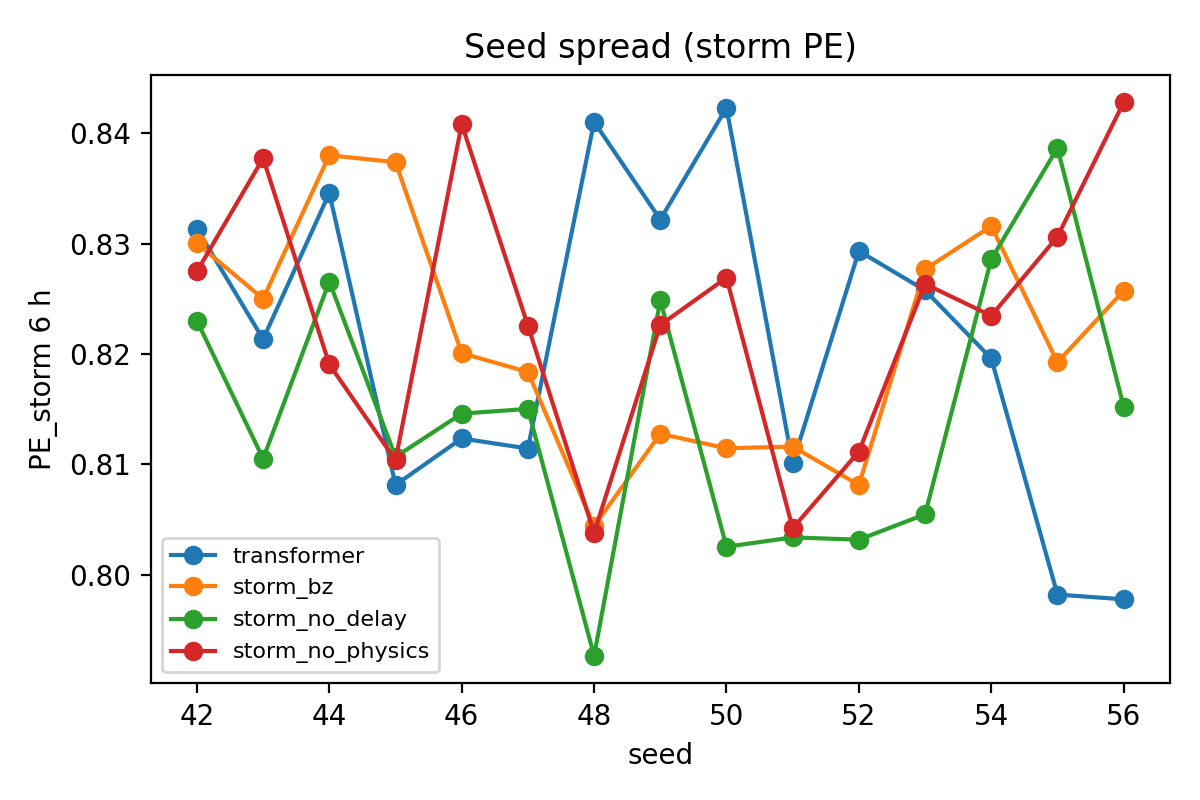
\includegraphics[width=\columnwidth]{figures/fig_seed_spread.png}
\caption{Seed-wise PE against climatology for Transformer and STORM-Bz
(seeds 42--56). Short-horizon STORM scores cluster tightly above the
Transformer; at 6\,h the two families overlap, consistent with the paired
tests in the text.}
\label{fig:seeds}
\end{figure}

\begin{figure*}[!htbp]
\centering

\includegraphics[width=0.75\textwidth]{figures/fig_ensemble_alpha_sweep.png}
\caption{Validation PE\textsubscript{6h} versus mixing weight \(\alpha\). Vertical line: \(\alpha^* = 0.3\) selected on validation; corresponding test PE is reported in Table~\ref{tab:main}.}
\label{fig:ensemble_sweep}
\end{figure*}

\begin{figure}[!htbp]
\centering

\includegraphics[width=\columnwidth]{figures/fig_horizon_pe.png}
\caption{Per-horizon PE against climatology (mean\(\pm\)std, fifteen seeds).
STORM-Bz leads at 45\,min; at 6\,h and 12\,h the single models are close,
while the ensemble improves multi-horizon PE (see Table~\ref{tab:main}).}
\label{fig:horizon}
\end{figure}



\subsection{Dst Intensity Bins}
Table~\ref{tab:dst} stratifies the full GOES--OMNI working sample by physical Dst for
STORM-Bz. Dst bins in Table~\ref{tab:dst} are a single-seed diagnostic and are not
seed-averaged like Table~\ref{tab:main}. Skill is about 0.76 on quiet hours, rises to about 0.79--0.80 on
minor and moderate storm bins, and remains about 0.71 on the sparse strong-storm
bin (\(\mathrm{Dst} \le -100\,\mathrm{nT}\), \(n=206\)). The model therefore does not rely
only on quiet persistence-dominated intervals.

\begin{table}[!htbp]
\centering
\caption{STORM-Bz 6\,h PE by Dst intensity\textsuperscript{a}}
\label{tab:dst}
\begin{tabular}{lcc}
\toprule
Intensity bin & Count & PE\(_{6\mathrm{h}}\) \\
\midrule
Quiet (\(\mathrm{Dst} > -30\)) & 77435 & 0.756 \\
Minor (\(-50 < \mathrm{Dst} \le -30\)) & 7127 & 0.793 \\
Moderate (\(-100 < \mathrm{Dst} \le -50\)) & 2316 & 0.800 \\
Strong (\(\mathrm{Dst} \le -100\)) & 206 & 0.708 \\
\bottomrule
\multicolumn{3}{p{0.95\columnwidth}}{\rule{0pt}{3ex}\textsuperscript{a}\footnotesize Full chronological GOES--OMNI working sample (includes training data, so this is a descriptive diagnostic, not test-set PE); single-seed diagnostic, not averaged across seeds.} \\
\end{tabular}
\end{table}

\begin{figure}[!htbp]
\centering
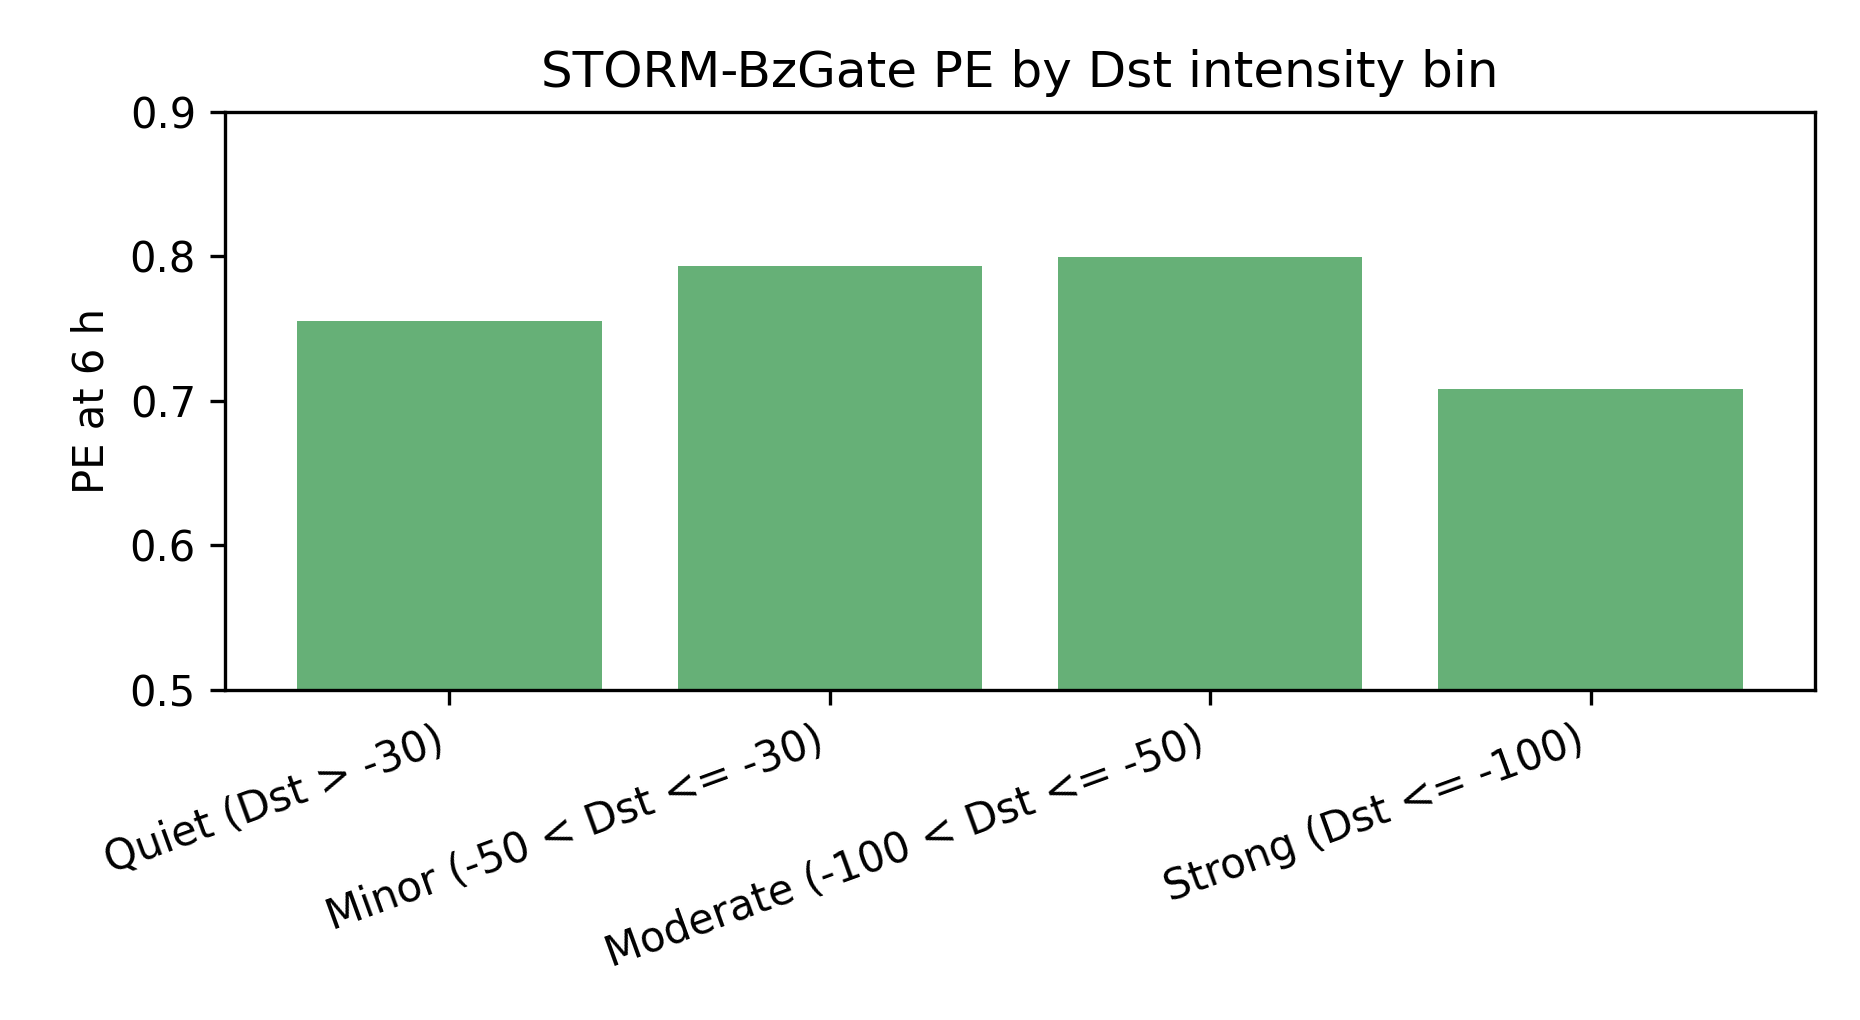
\includegraphics[width=\columnwidth]{figures/fig_dst_bins.png}
\caption{STORM-Bz 6\,h PE stratified by Dst intensity bin on the full GOES--OMNI working sample. \textbf{Note: this includes training data and is a descriptive diagnostic, not test-set PE.}}
\label{fig:dst}
\end{figure}

\subsection{Input Noise and Missing Channels}
Gaussian noise was added to standardized solar-wind inputs at test time
(\(\sigma\in\{0,0.2,0.5,1.0,1.5,2.0\}\)) for Transformer, STORM-Bz,
hybrid, and ensemble systems over fifteen seeds.
At \(\sigma=2\), Transformer PE\(_{45\mathrm{min}}\) falls from about
\(0.96\) to about \(0.61\), whereas STORM remains near \(0.96\).
At 6\,h the ensemble and STORM also lose less skill than the Transformer.
Zeroing feature groups (no \(B_z\); no velocity/density; no rolling
averages) produces the same qualitative ordering (detailed tables provided in the accompanying code repository): STORM holds
PE\(_{45\mathrm{min}}\) near \(0.986\mbox{--}0.987\) while the Transformer drops more
when derived rolling channels are removed.
These checks are controlled diagnostics, not a claim of immunity to
arbitrary sensor failure.

\begin{figure*}[!htbp]
\centering
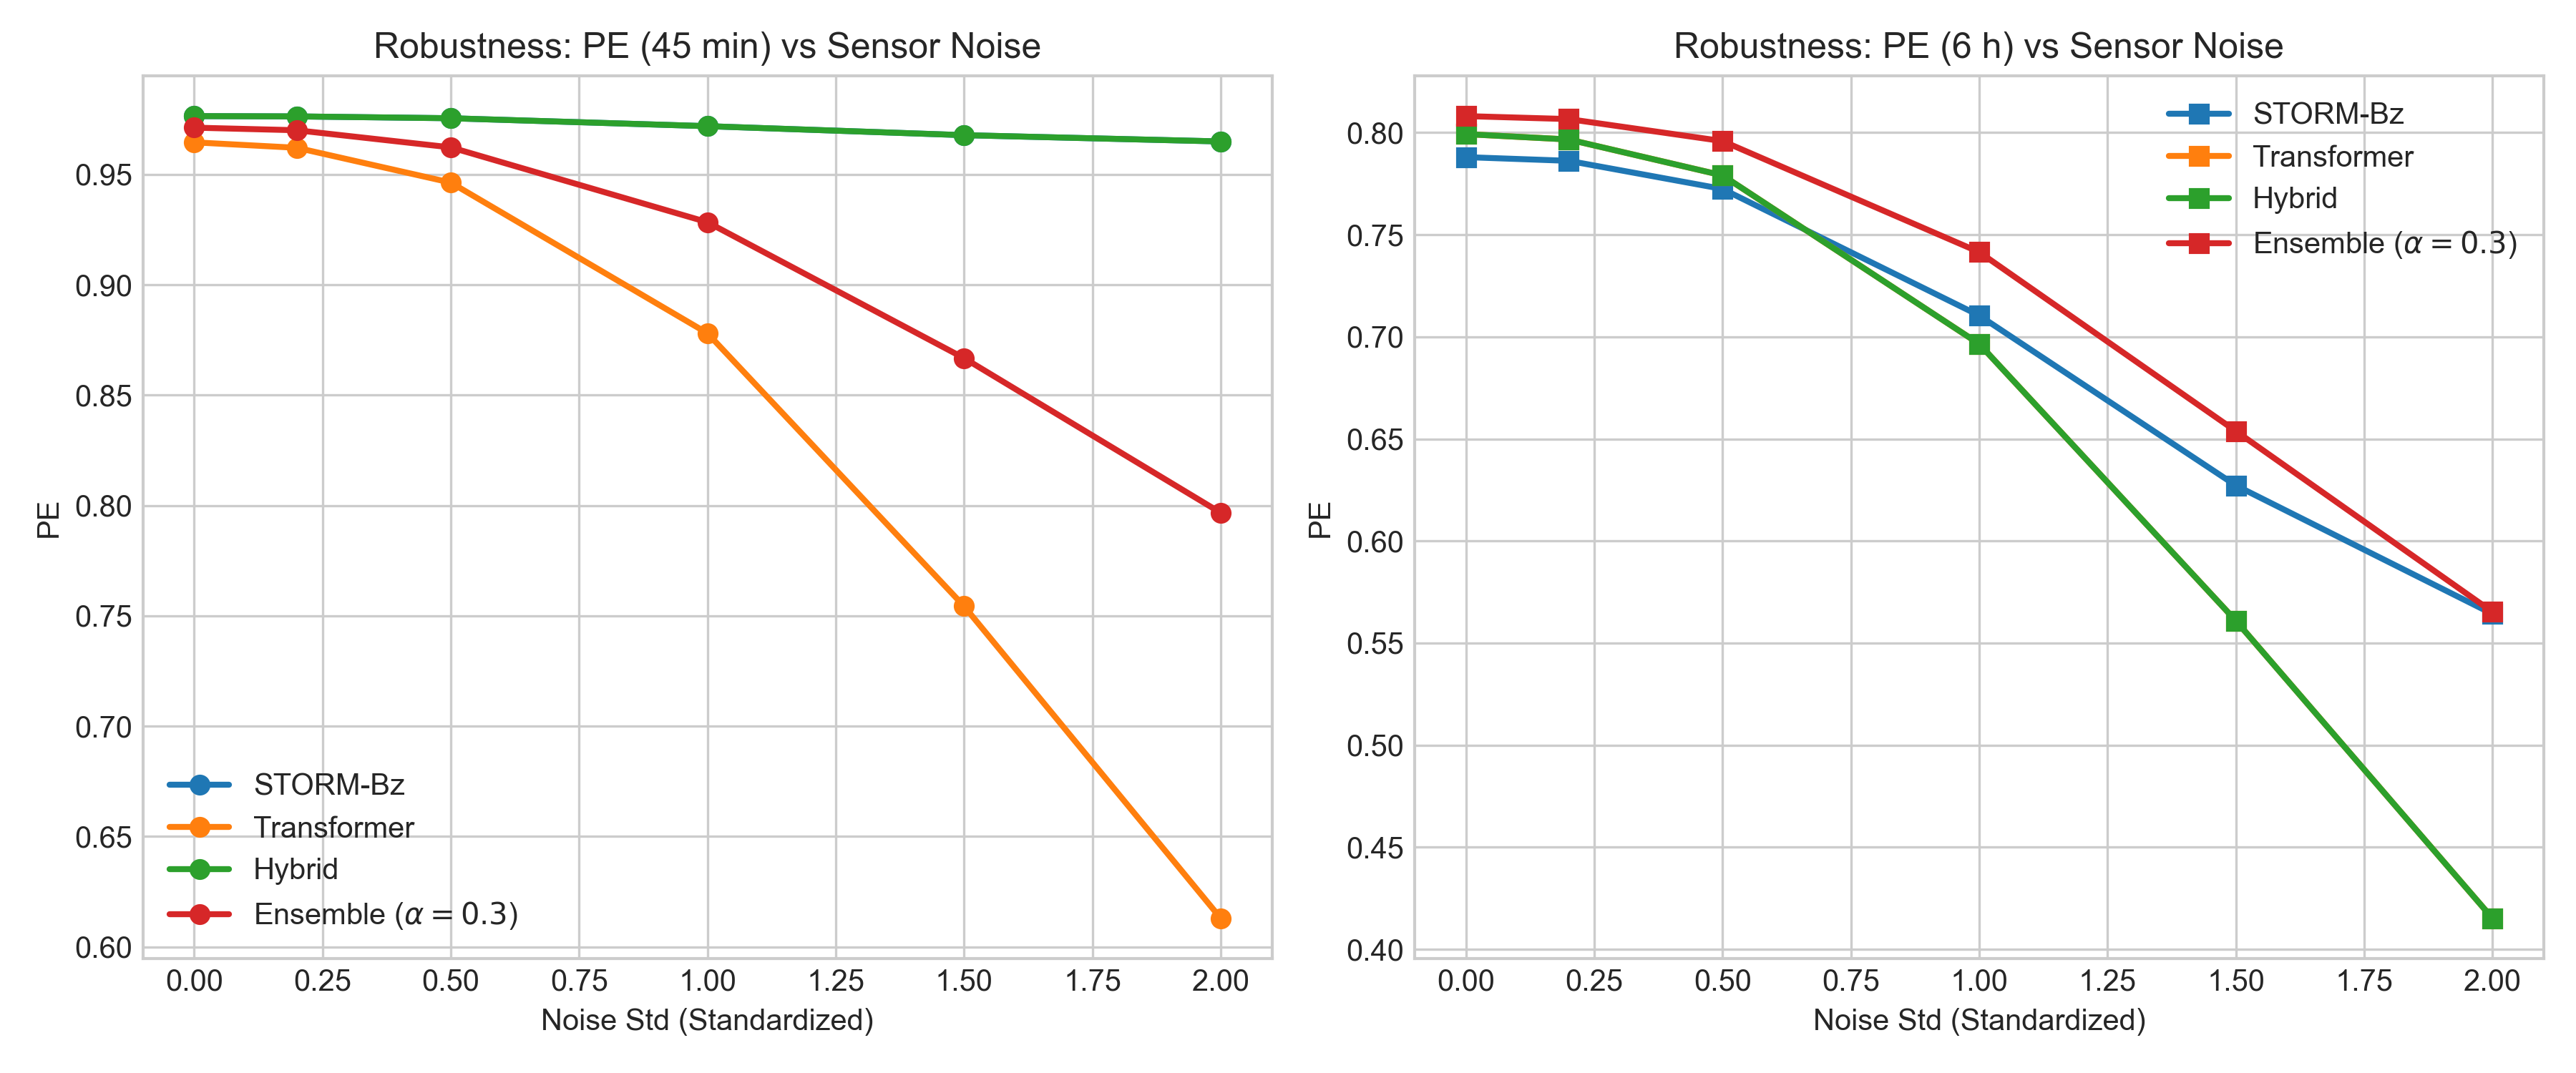
\includegraphics[width=0.75\textwidth]{figures/noise_robustness.png}
\caption{Prediction efficiency under Gaussian noise on standardized solar-wind
inputs (fifteen seeds). STORM and hybrid retain short-horizon PE under strong
noise; the Transformer degrades sharply at 45\,min. Ensemble remains competitive
at moderate noise levels.}
\label{fig:noise}
\end{figure*}


\subsection{Compute Cost}
Table~\ref{tab:compute} reports parameter counts and batch-32 GPU latency in our
timing setup. STORM-Bz is lighter than the Transformer baseline while remaining
competitive on all-hour 6\,h PE and improving short-horizon reliability. As noted in Section~\ref{sec:method}, measured parameter counts are approximately $3.43\times10^{5}$ for STORM-Bz and $8.45\times10^{5}$ for the Transformer baseline; the two models are not capacity-matched.

\begin{table}[!htbp]
\centering
\caption{Model size and inference cost (batch 32, GPU, single seed)}
\label{tab:compute}
\begin{tabular}{lcc}
\toprule
Model & Parameters & ms / batch \\
\midrule
Transformer (baseline) & \(8.45\times10^{5}\) & 2.95 \\
STORM-Bz & \(3.43\times10^{5}\) & 3.73 \\
\bottomrule
\end{tabular}
\end{table}

The delay-module interpolation introduces a sequential operation not present in
the pure Transformer, which accounts for the modest per-batch latency increase
despite the smaller parameter count.

\begin{figure*}[!htbp]
\centering
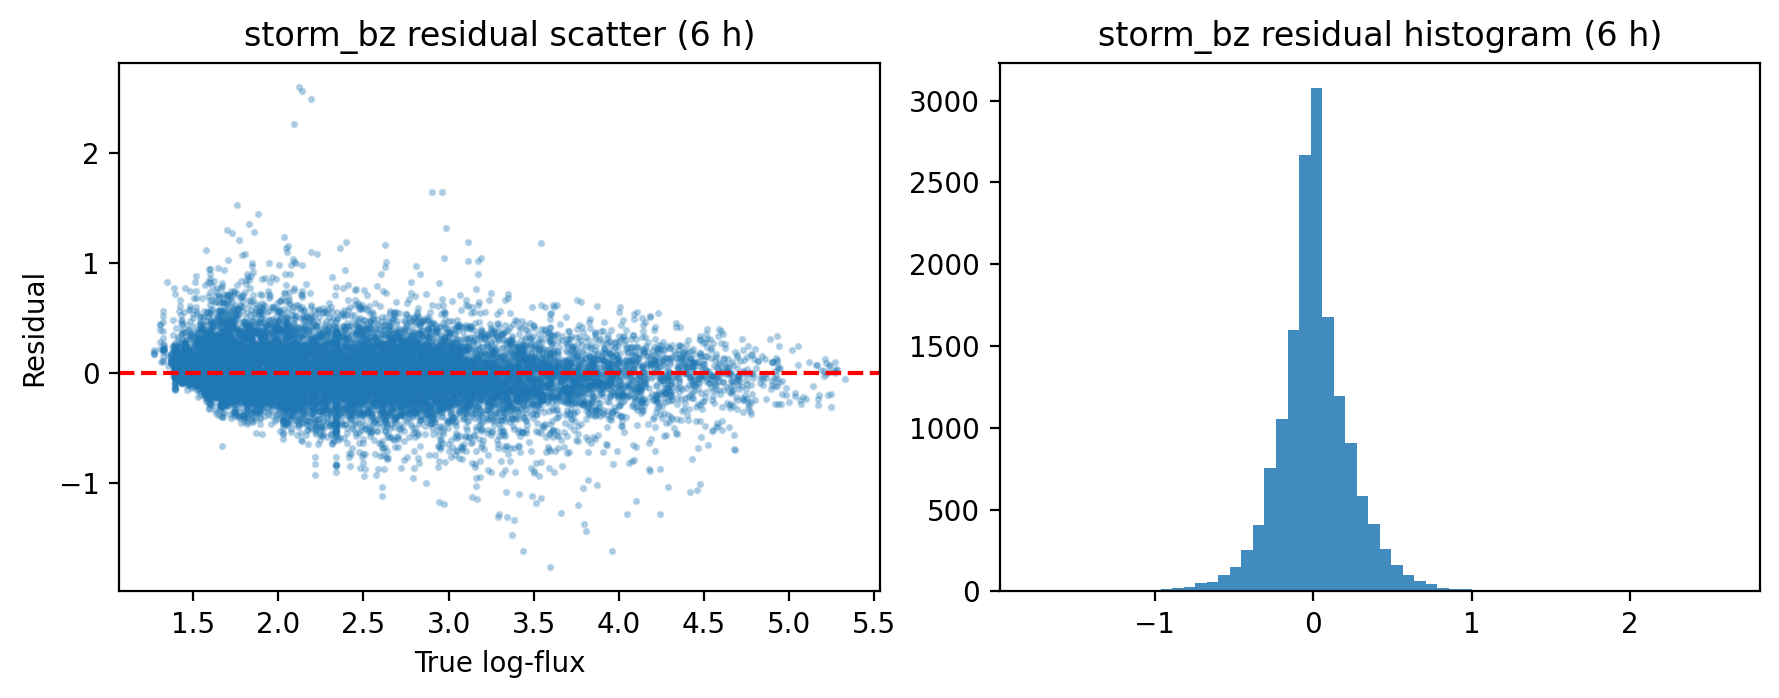
\includegraphics[width=0.65\textwidth]{figures/fig_residual_storm_bz.png}
\caption{Residual distribution (predicted minus true log-flux) for STORM-Bz
on the GOES test set, stratified by storm and quiet windows.}
\label{fig:resid_storm}
\end{figure*}

\begin{figure*}[!htbp]
\centering
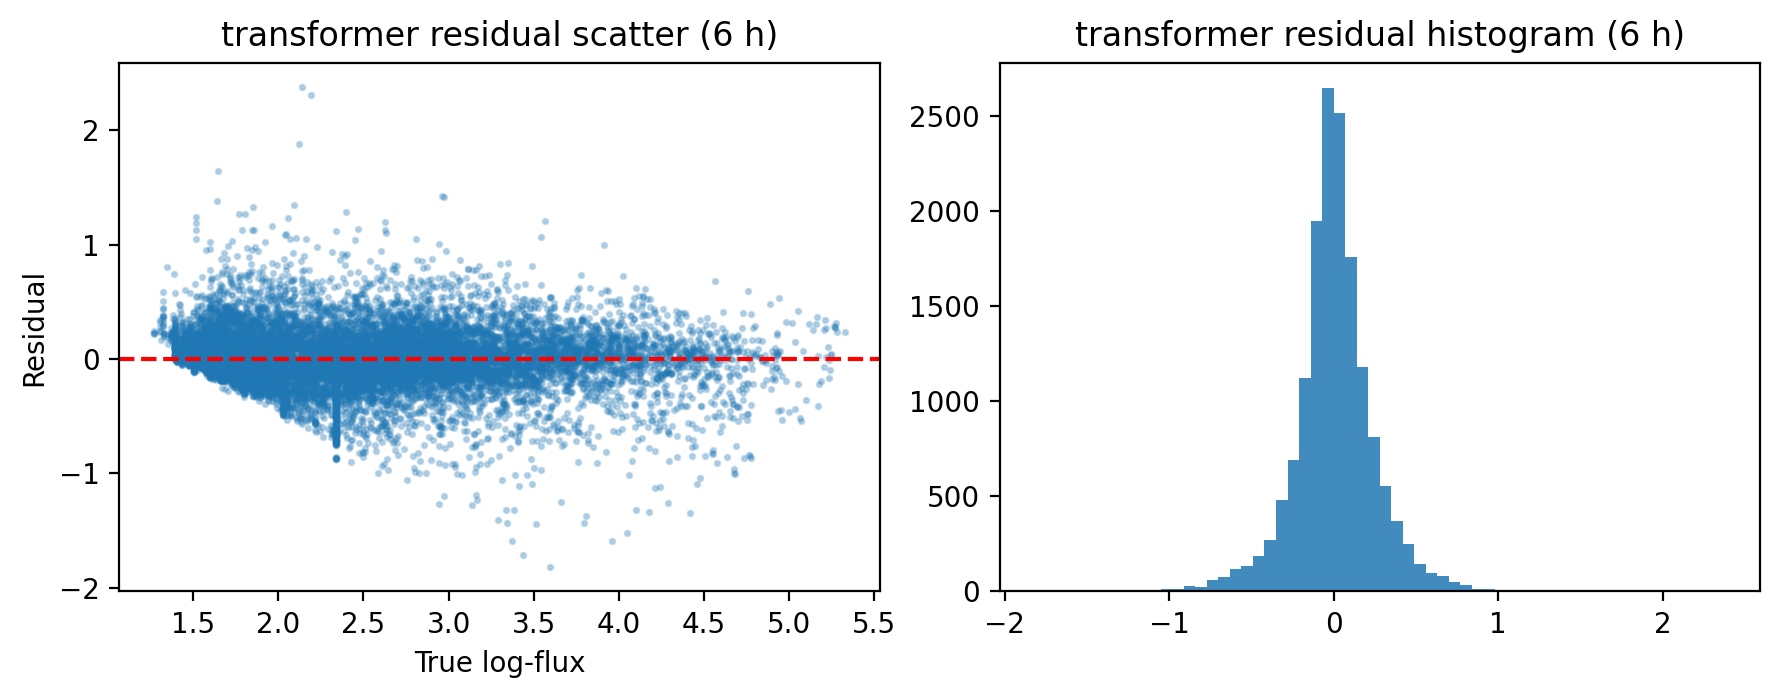
\includegraphics[width=0.65\textwidth]{figures/fig_residual_transformer.png}
\caption{Same residual view for the Transformer baseline.}
\label{fig:resid_tf}
\end{figure*}

\subsection{Event Time Series}
Fig.~\ref{fig:case_enhancement} shows STORM-Bz predictions against observed log-flux
during a major flux enhancement event in the GOES test period. The model captures
the broad shape of the multi-day enhancement and recovery more closely than persistence. We do not claim the gate panel tracks reconnection from these plots alone. The model struggles with sharp dropout and quiet conditions (Fig.~\ref{fig:case_dropout} and Fig.~\ref{fig:case_quiet}), which are included as failure modes rather than success cases.

\begin{figure*}[!htbp]
\centering
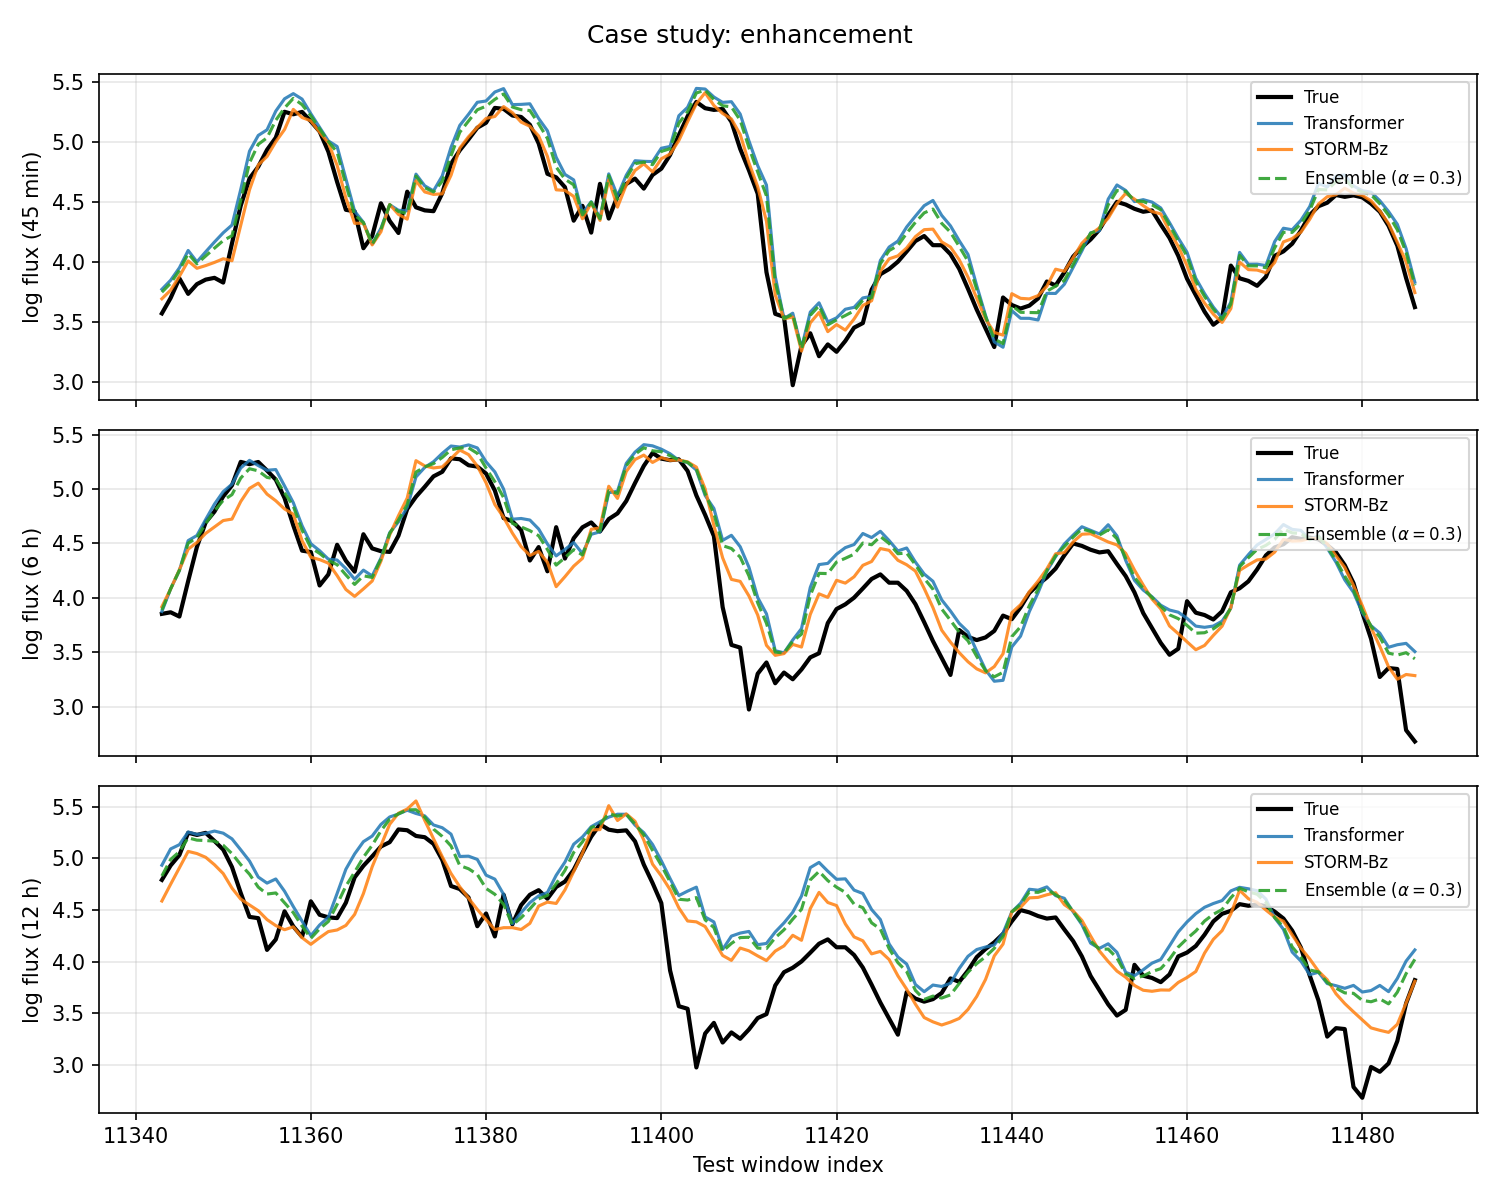
\includegraphics[width=0.65\textwidth]{figures/fig_case_enhancement.png}
\caption{Illustrative enhancement window. Top: true log-flux, STORM-Bz, and persistence. Lower panels: Bz, Vsw, predicted \(\tau\), and gate. \(\tau\) is constrained to \([0.5, 1.5]\) h.}
\label{fig:case_enhancement}
\end{figure*}

\begin{figure*}[!htbp]
\centering
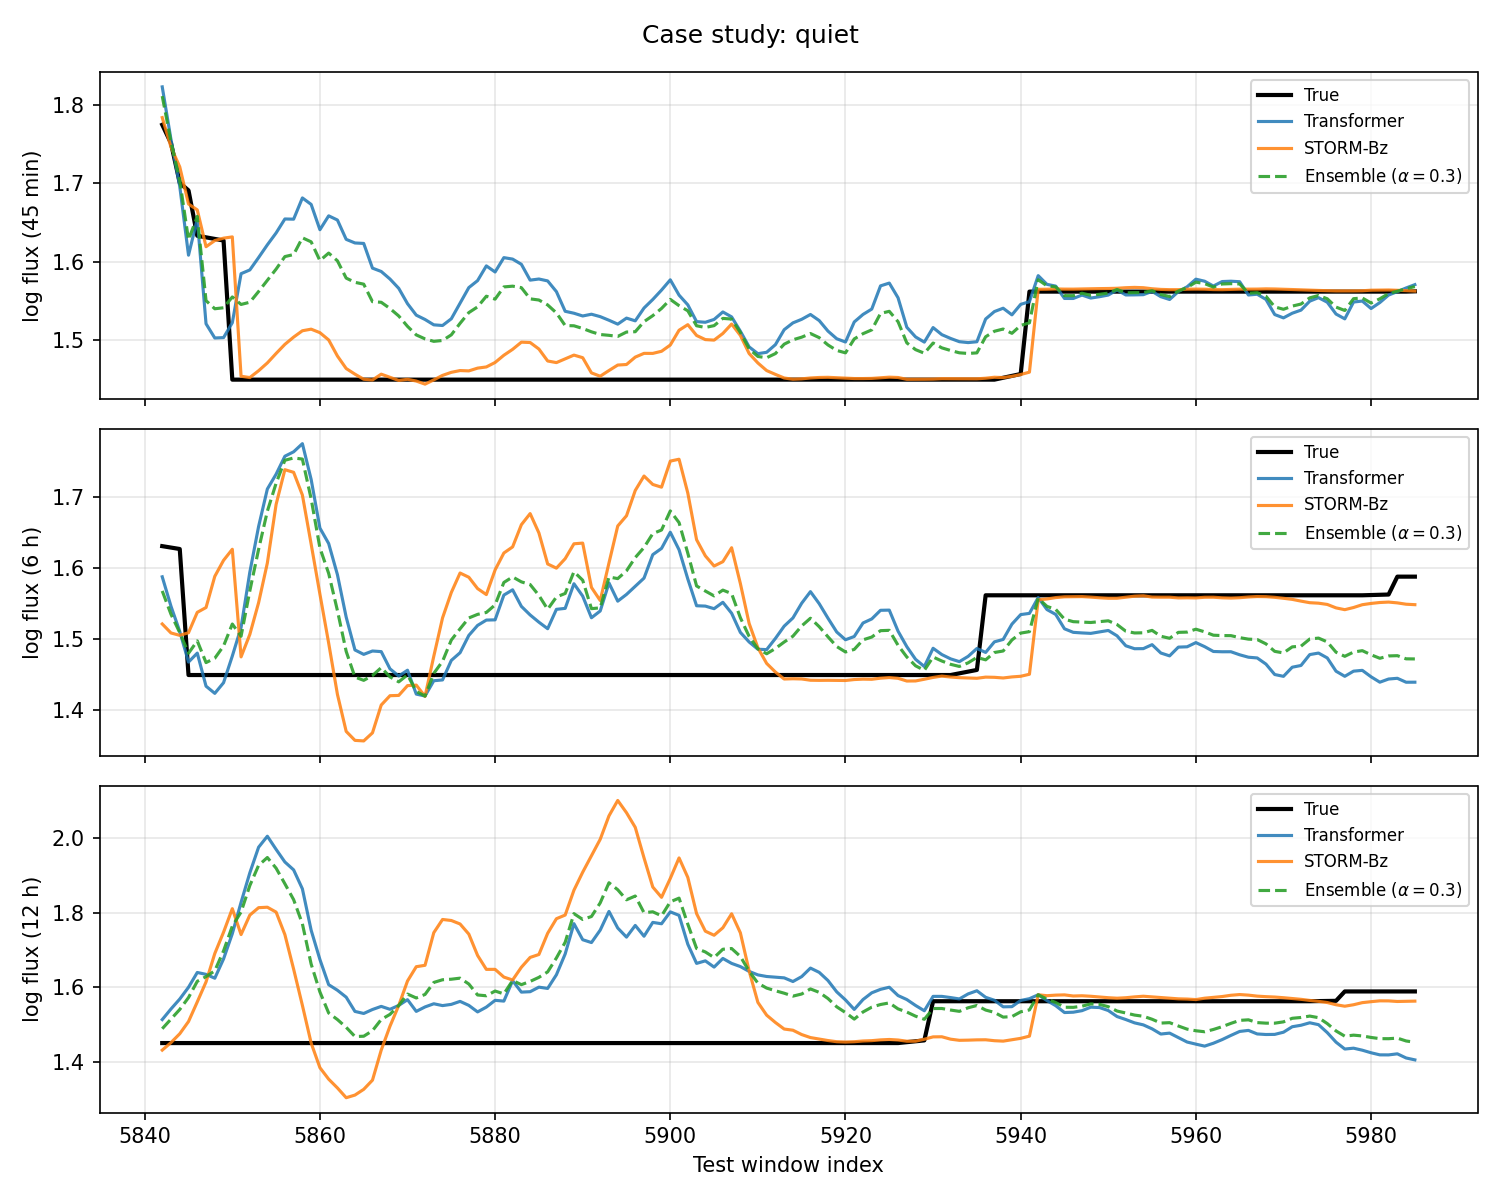
\includegraphics[width=0.65\textwidth]{figures/fig_case_quiet.png}
\caption{Quiet drift failure mode. The model overpredicts gradual flux recovery during low geomagnetic activity.}
\label{fig:case_quiet}
\end{figure*}

\begin{figure*}[!htbp]
\centering
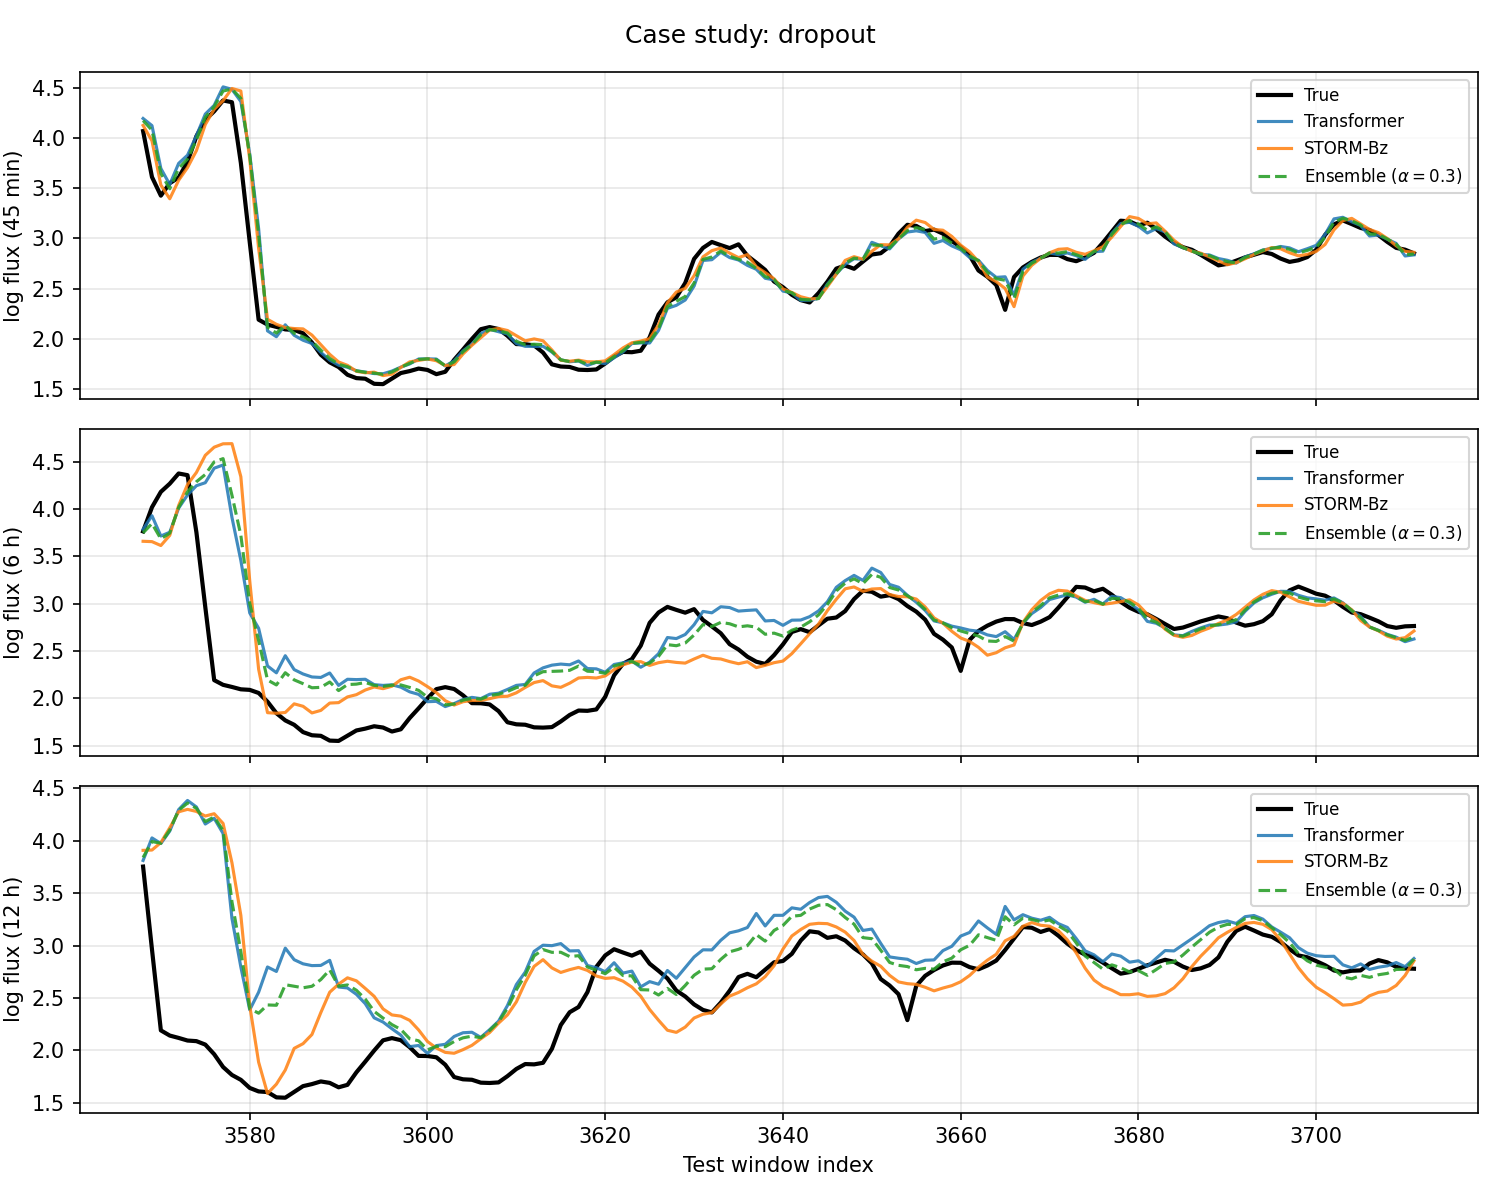
\includegraphics[width=0.65\textwidth]{figures/fig_case_dropout.png}
\caption{Sharp dropout failure mode. The model does not fully capture the rapid magnetopause shadowing flux drop.}
\label{fig:case_dropout}
\end{figure*}

\subsection{Residual structure}
Residual histograms (Figs.~\ref{fig:resid_storm}--\ref{fig:resid_tf}) show
that errors concentrate near zero on quiet hours and widen in storm windows
for both models; STORM does not eliminate storm-time residual variance, but
it reduces the short-horizon bias relative to persistence discussed above.

\subsection{Interpretability}
\begin{figure}[!htbp]
\centering
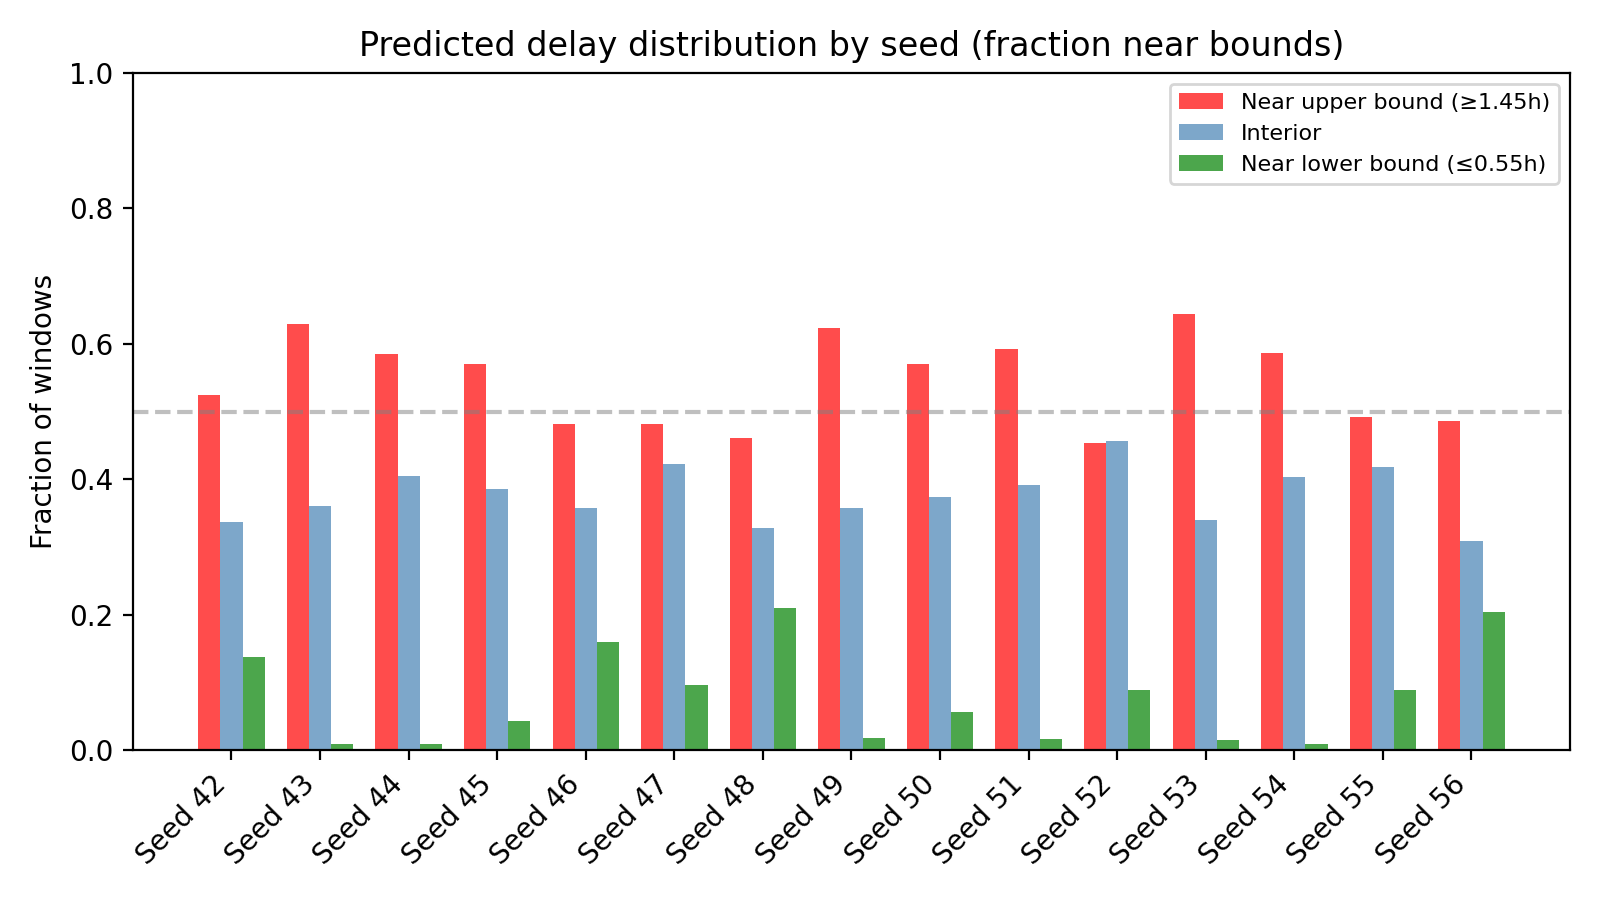
\includegraphics[width=\columnwidth]{figures/fig_physics_tau_hist.png}
\caption{Fraction of predicted propagation delays \(\tau\) near the constraint bounds across fifteen seeds. The blue bars show the interior fraction, red bars show the fraction near the upper bound (\(1.5\,\mathrm{h}\)), and green bars show the fraction near the lower bound (\(0.5\,\mathrm{h}\)). The saturation at the upper bound indicates the box constraint is active.}
\label{fig:delay}
\end{figure}

\begin{figure}[!htbp]
\centering
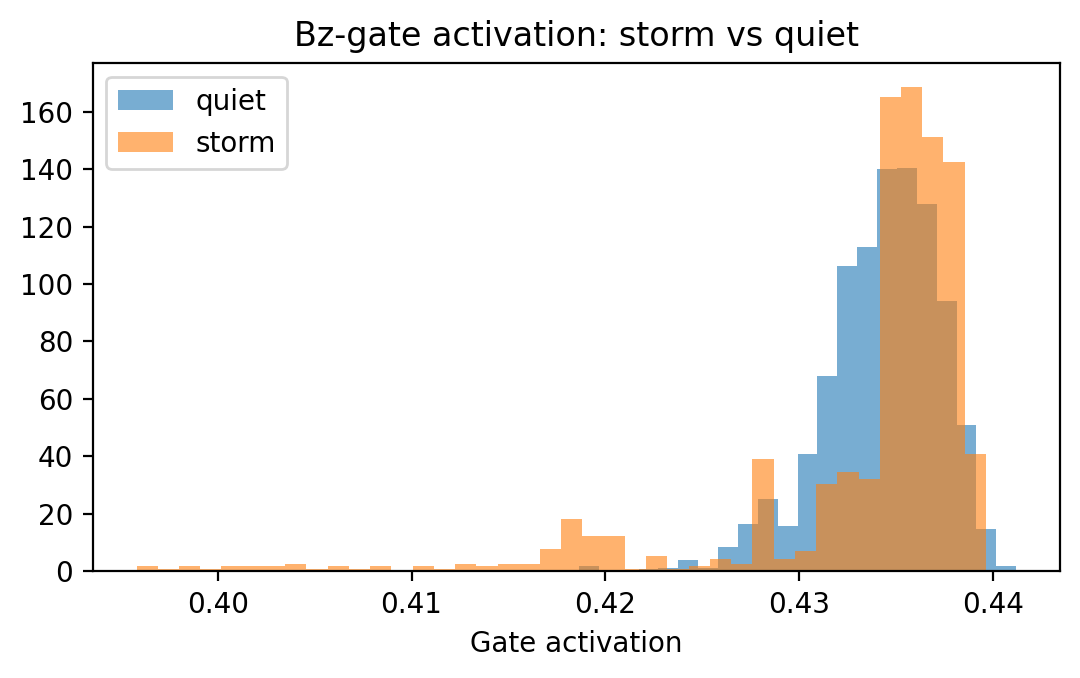
\includegraphics[width=\columnwidth]{figures/fig_physics_gate_storm_quiet.png}
\caption{\(B_z\) gate activation: storm windows (orange) versus quiet intervals
(blue) (Mann--Whitney \(p = 1.2\times10^{-14}\)).}
\label{fig:gate}
\end{figure}

Fig.~\ref{fig:physics_scatter} relates the two trainable physics modules to
familiar solar-wind drivers; these panels are diagnostic, not a claim that
\(\tau\) recovers a unique physical constant on every window.

\begin{figure}[!htbp]
\centering
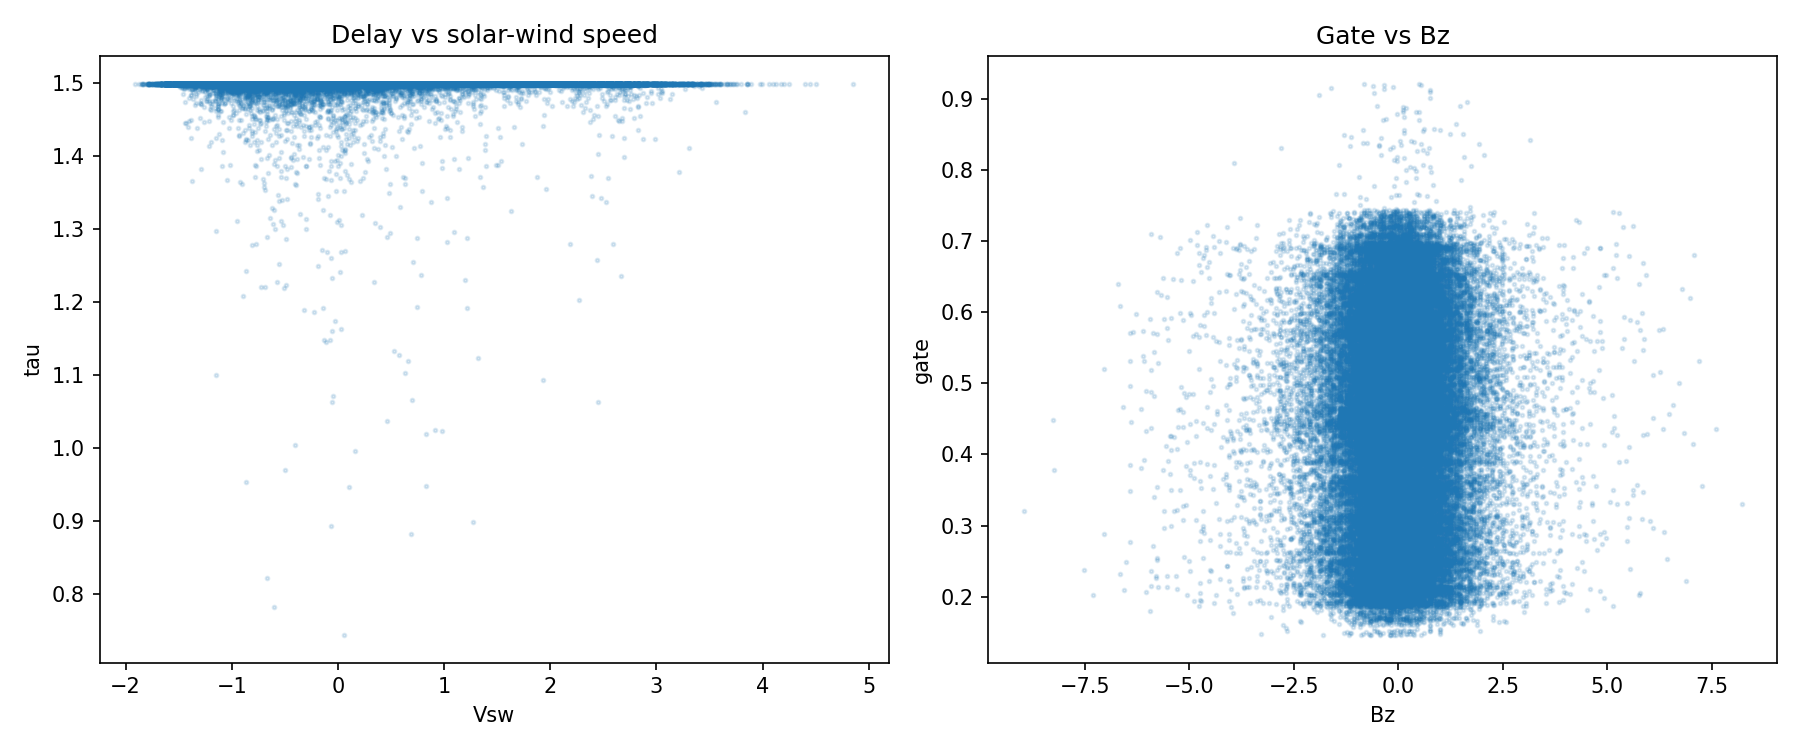
\includegraphics[width=\columnwidth]{figures/physics_scatters.png}
\caption{Physics-module diagnostics on the GOES test set: predicted delay
\(\tau\) against solar-wind speed, and gate activation against southward
\(B_z\) statistics. Delays remain inside the imposed \([0.5,1.5]\,\mathrm{h}\)
band; gate values rise when southward IMF is sustained.}
\label{fig:physics_scatter}
\end{figure}

\begin{figure}[!htbp]
\centering

\includegraphics[width=\columnwidth]{figures/fig_feature_importance.png}
\caption{Permutation importance on the \(6\,\mathrm{h}\) head for STORM-Bz
(PE drop when each input channel is shuffled). \(B_z\) and related solar-wind
drivers rank highest.}
\label{fig:perm}
\end{figure}

\subsection{GRASP Transfer}
On GSAT-19 GRASP (fifteen seeds), zero-shot GOES models already achieve
short-horizon PE near \(0.82\), but 6\,h and 12\,h PE fall. Fine-tuning on GRASP (freezing the Transformer encoder and updating only the forecast heads) raises 6\,h PE from 0.449 to 0.599 (paired \textit{t}-test across fifteen seeds, \(p = 7.6\times10^{-7}\), Cohen's \(d = 2.17\)) and 12\,h PE from 0.182 to 0.517 (\(p = 3.6\times10^{-10}\), \(d = 3.98\)).
The inter-seed standard deviation after fine-tuning remains 0.073 at both 6\,h
and 12\,h, indicating that transfer convergence is still seed-sensitive; future
work should examine learning-rate schedules specific to the fine-tuning stage.
Absolute GRASP PE remains below
the GOES test scores, as expected under sensor and longitude shift; the
practical point is the large mid- and long-horizon recovery after
adaptation rather than a claim of parity with GOES.

\begin{table*}[!htbp]
\centering
\caption{GRASP (GSAT-19) transfer results (fifteen seeds). Paired tests across fifteen seeds are reported in the text. Bold: best per horizon.}
\label{tab:grasp}
\begin{tabular}{lccc}
\toprule
Horizon & Zero-shot & Fine-tuned & Gain \\
\midrule
\(\approx\)45\,min & 0.820 $\pm$ 0.001 & 0.827 $\pm$ 0.009 & +0.007 \\
6 h & 0.449 $\pm$ 0.011 & \textbf{0.599 $\pm$ 0.073} & \textbf{+0.150} \\
12 h & 0.182 $\pm$ 0.045 & \textbf{0.517 $\pm$ 0.073} & \textbf{+0.335} \\
\bottomrule
\end{tabular}
\end{table*}

\subsection{Horizon-Restricted Physics Loss}
We also trained a variant that applies physics-loss terms only on the
short head (ignoring the 6\,h and 12\,h heads).
Across fifteen seeds this variant did not differ significantly from the
baseline STORM model on PE\(_{6\mathrm{h}}\) (paired \(p\approx0.64\)).
We therefore treat horizon-restricted physics weighting as a null ablation
rather than a performance lever.

We further trained a No-Gate variant that sets the modulation
to identity (\(g=1\)). On PE\(_{\mathrm{clim}}\), removing the gate
does not reduce 45\,min skill relative to full STORM-Bz
(\(0.987\) versus \(0.986\) in Table~\ref{tab:main}); the same
null result holds for the No-Delay and No-Physics
ablations. The short-horizon gain versus the Transformer
is therefore a property of the trained STORM package under our
protocol, not a gain that disappears when any one physics module is
removed. We do not attribute that 45\,min PE\(_{\mathrm{clim}}\) edge
to the gate alone.

On storm windows, single-model PE\(_{\mathrm{st},6\mathrm{h}}\) values are close:
STORM-Bz \(0.827\), LSTM \(0.827\), Transformer \(0.821\), with
No-Delay and No-Physics slightly lower
(\(0.823\) and \(0.824\)) and No-Gate comparable or slightly
higher (\(0.829\)). Given overlapping intervals, we do not claim that
any one physics module is required for storm-time skill. The clearest
gains on storm subsets remain post-hoc aggregation: the
\(\alpha^*=0.3\) ensemble reaches \(0.839\) and seed-bagged STORM
reaches \(0.849\) (Table~\ref{tab:main}).

Fig.~\ref{fig:ablation} summarizes the same controlled comparison at 6\,h:
ablating delay or physics loss does not overturn the ranking already reported
in Table~\ref{tab:main}.

\begin{figure}[!htbp]
\centering
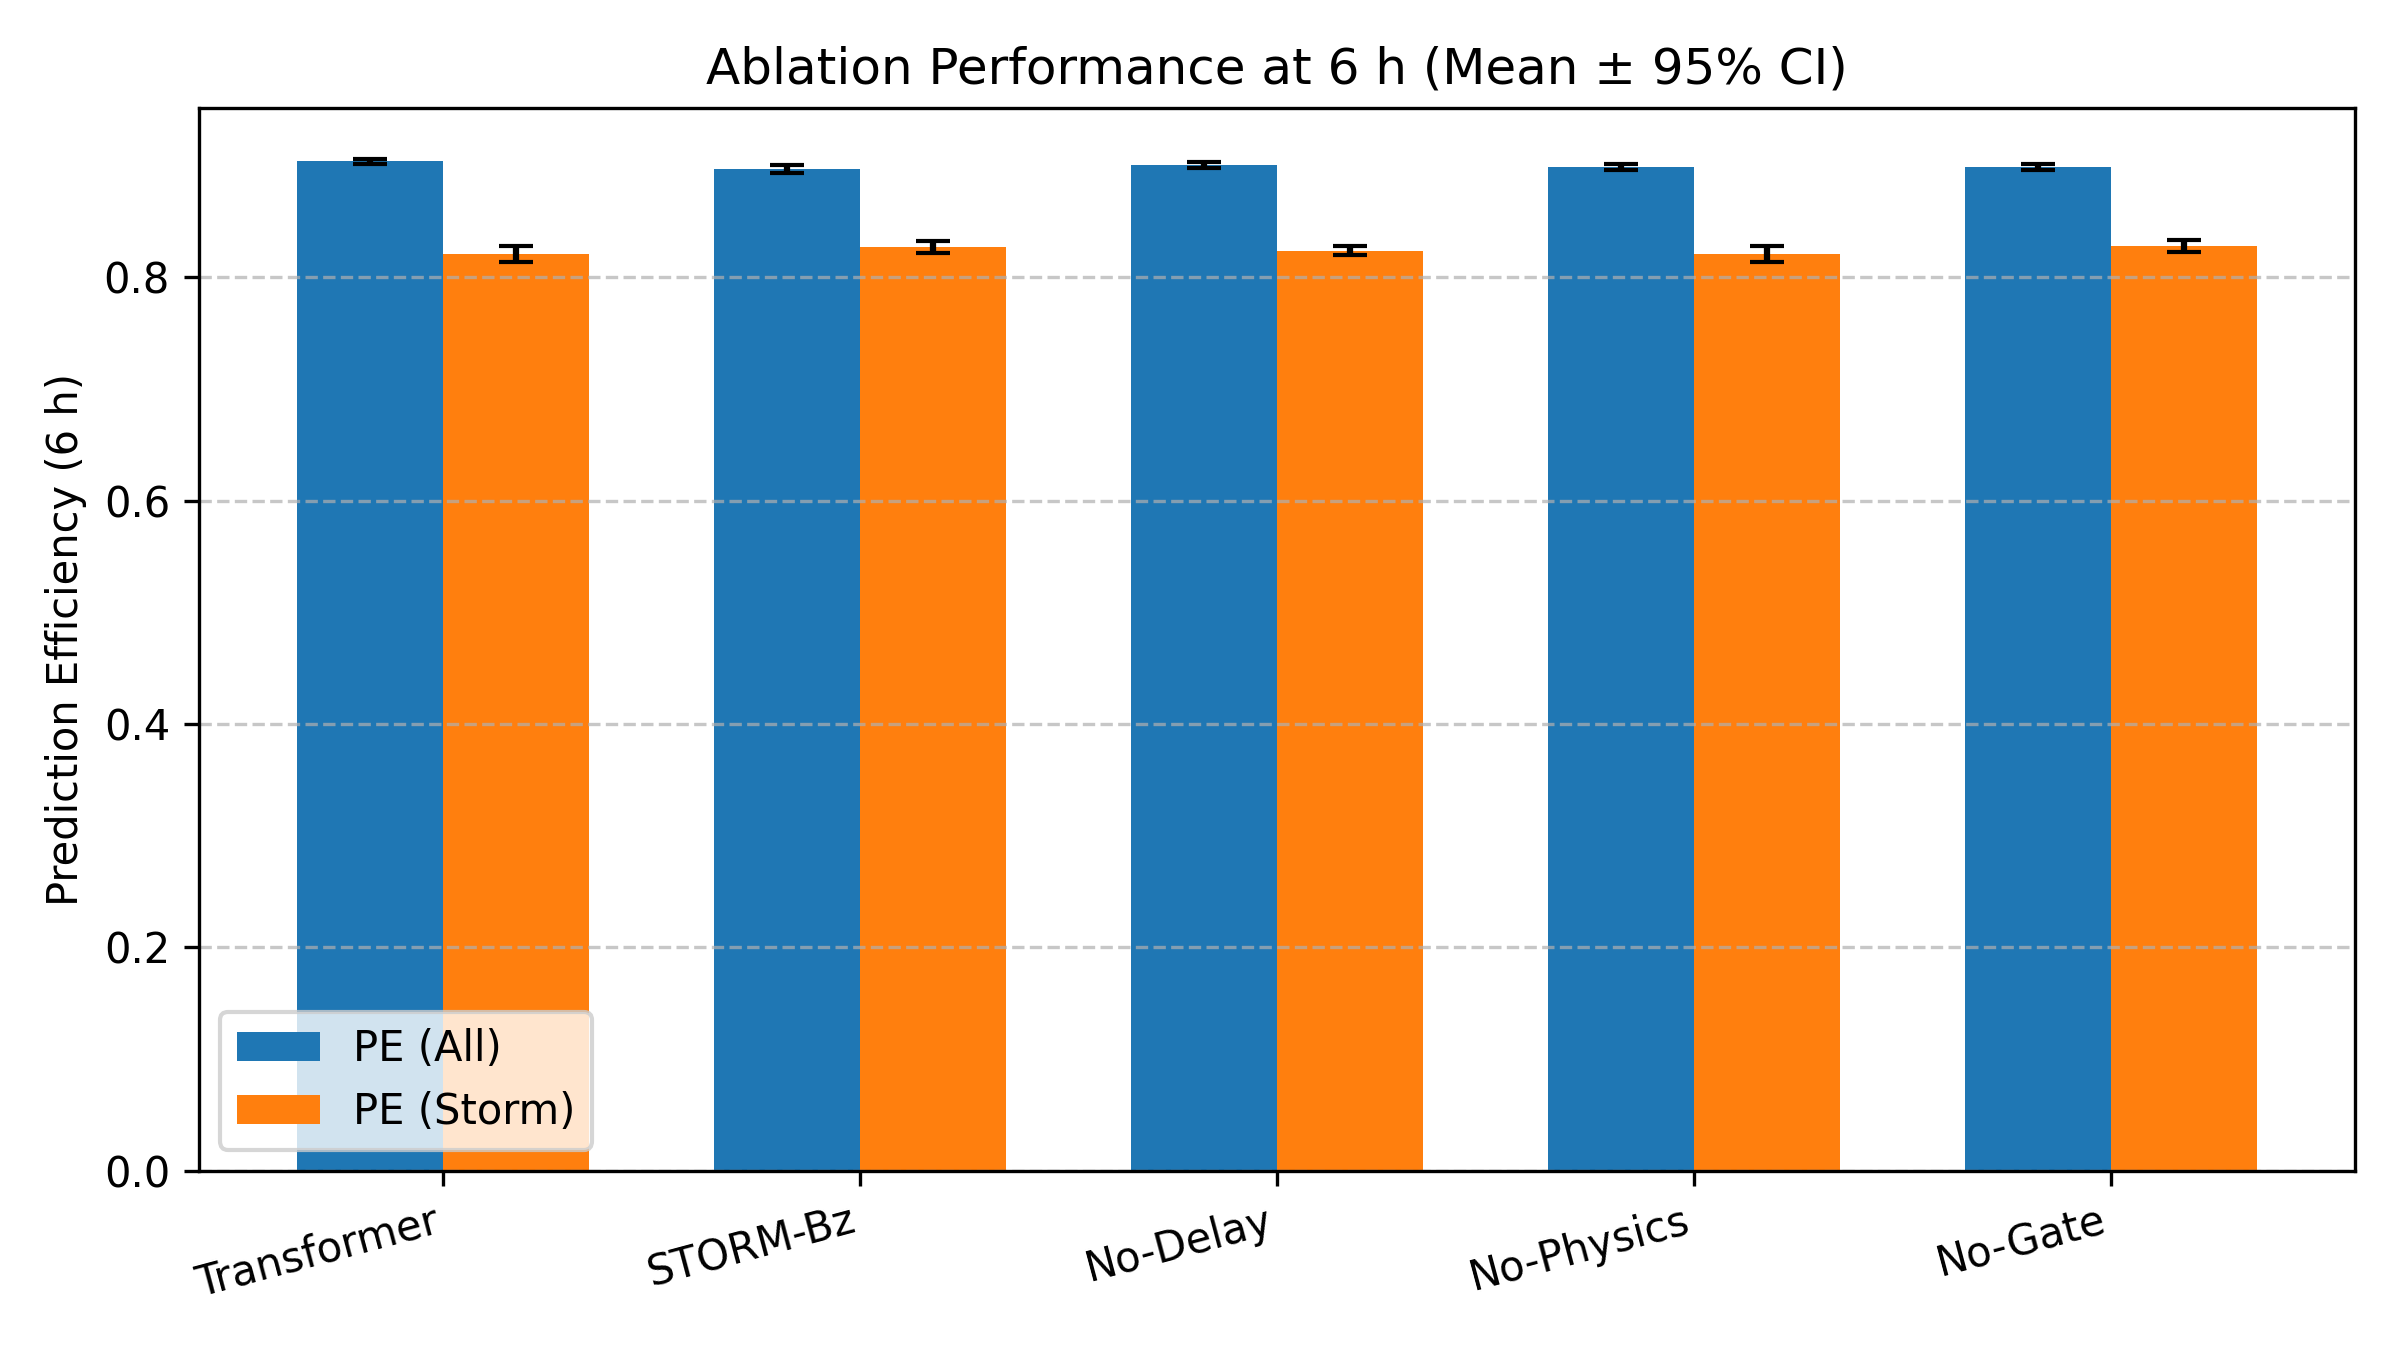
\includegraphics[width=\columnwidth]{figures/fig_ablation_6h.png}
\caption{Six-hour PE against climatology for the Transformer baseline,
full STORM-Bz, and ablations that remove the delay module or the physics-loss
term (fifteen seeds; mean\(\pm\)std). Removing the delay module, the physics-loss term, or the \(B_z\) gate
does not collapse PE\(_{6\mathrm{h}}\) or remove the 45\,min advantage
over the Transformer; the main single-model STORM advantage remains
the short-horizon comparison in Table~\ref{tab:main}.}
\label{fig:ablation}
\end{figure}

\begin{figure}[!htbp]
\centering
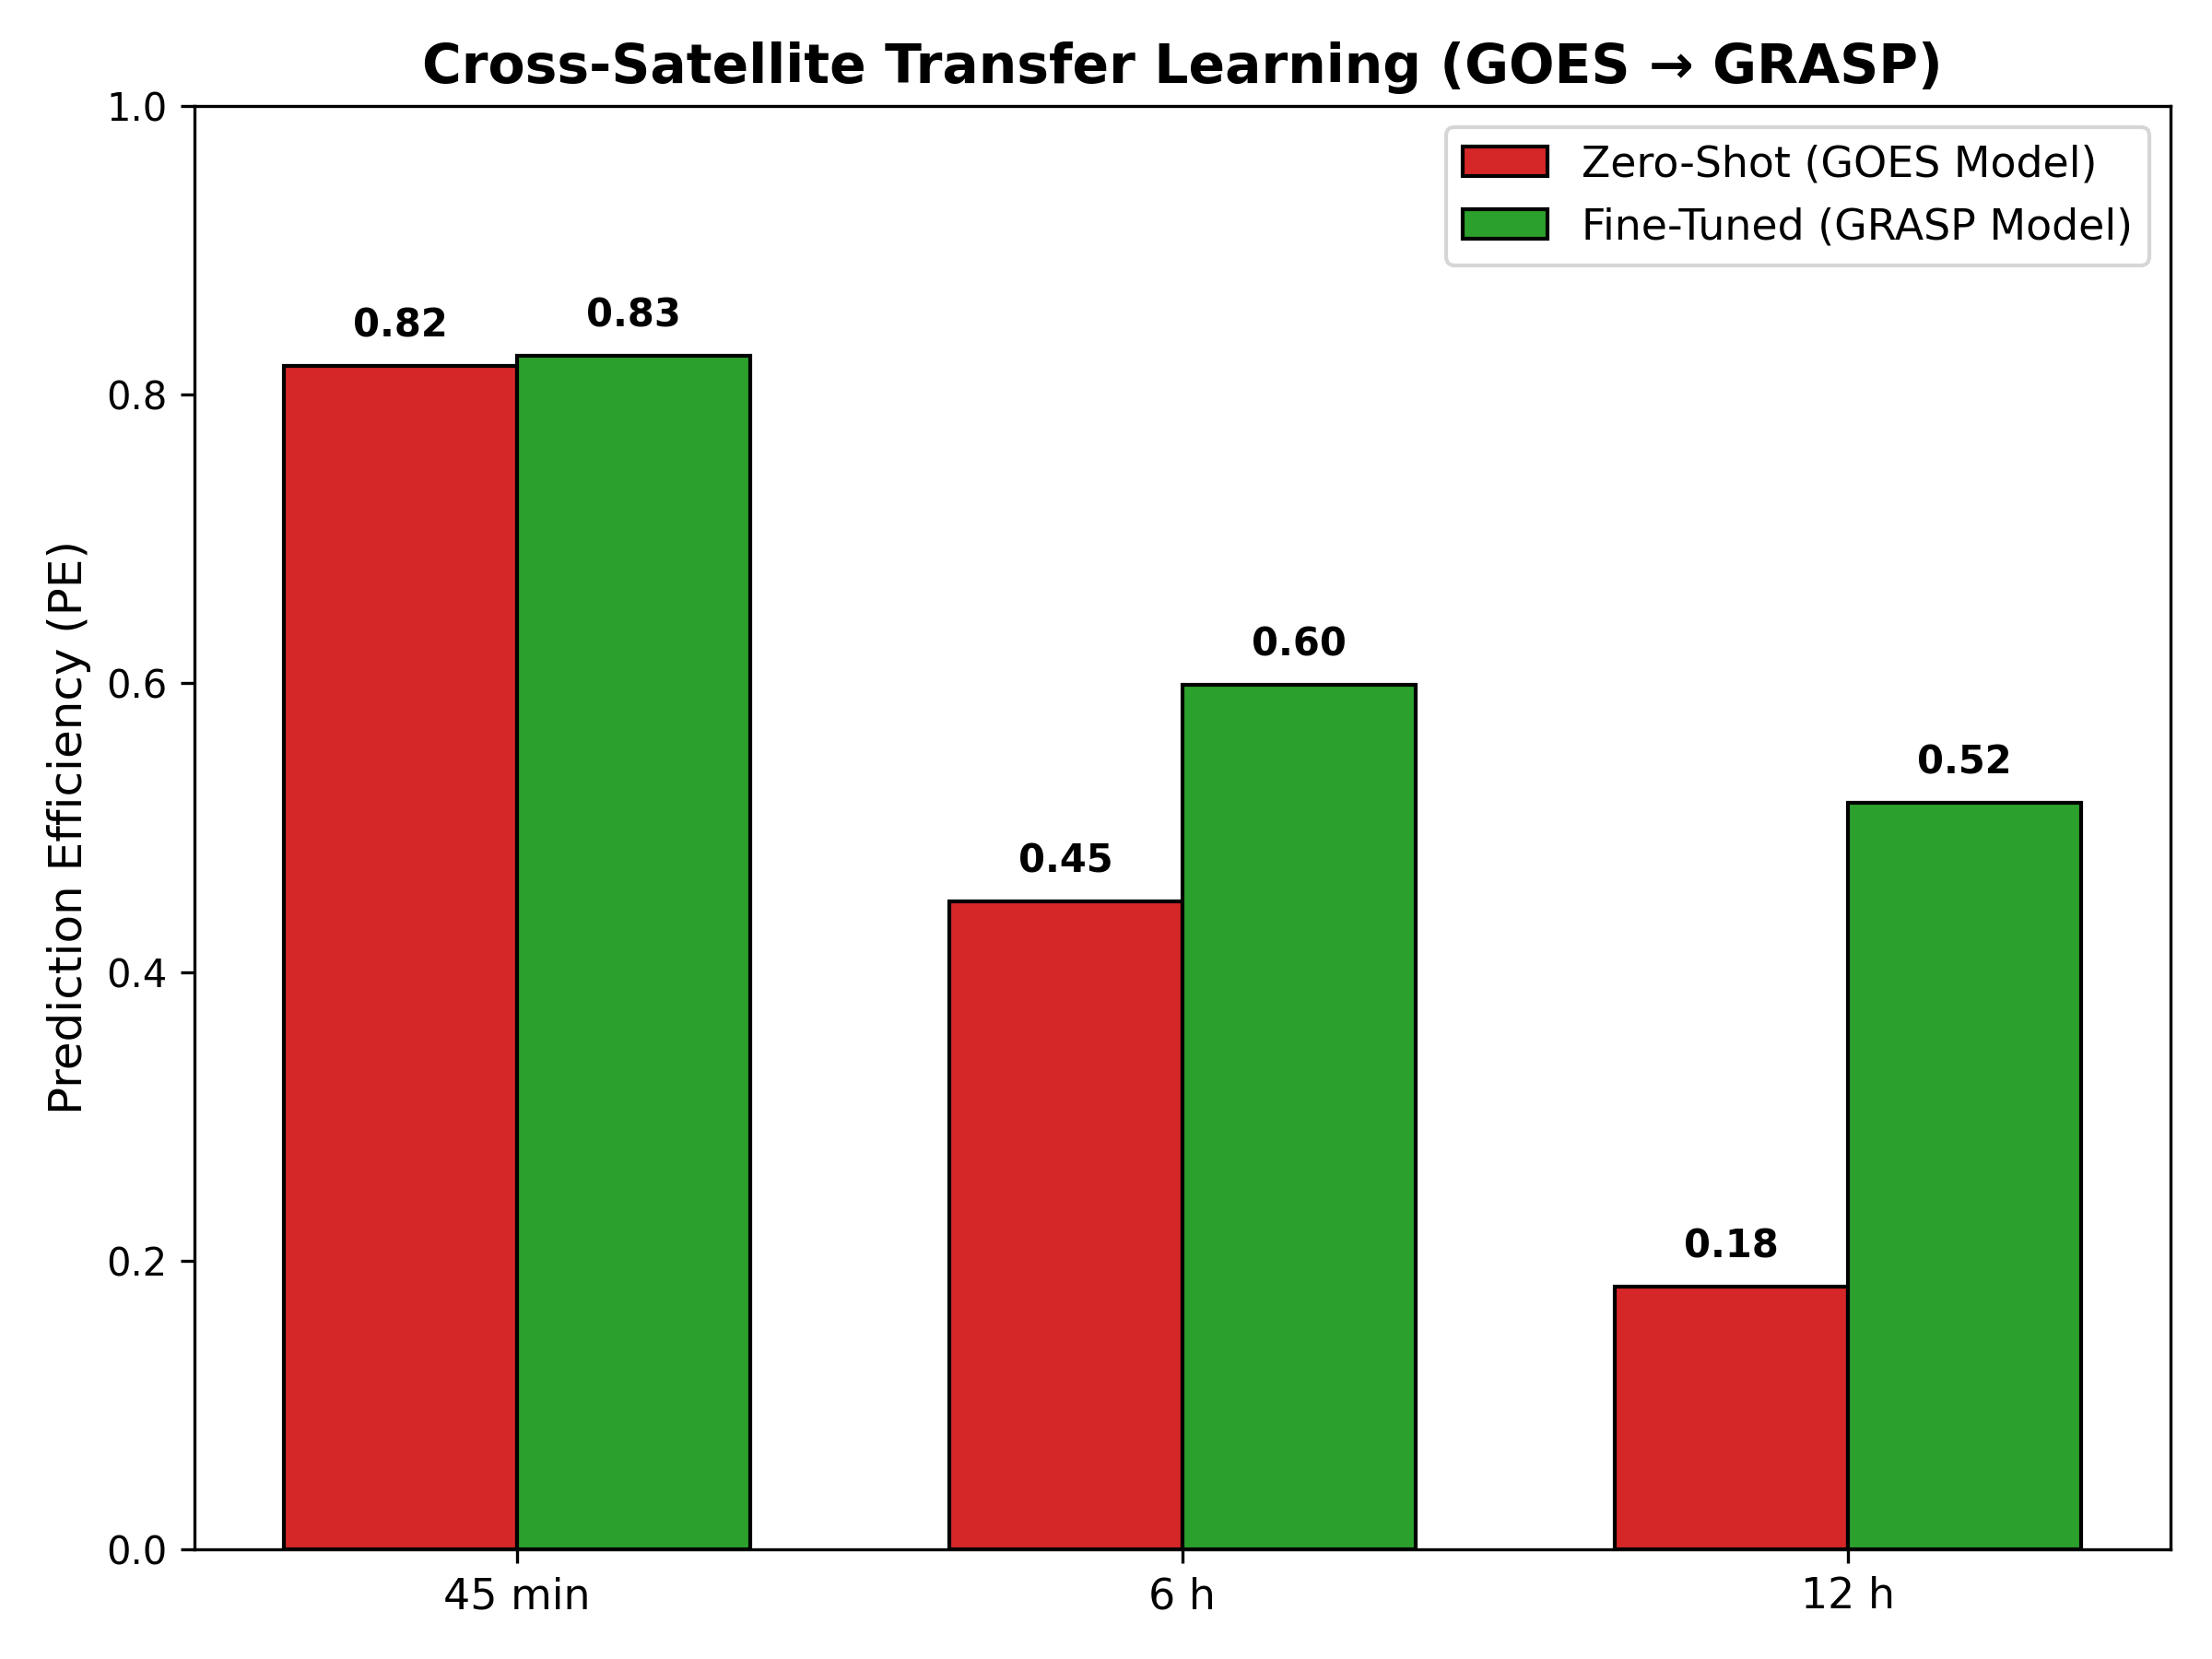
\includegraphics[width=\columnwidth]{figures/domain_gap_plot.png}
\caption{GRASP domain-gap summary (fifteen seeds): zero-shot GOES models versus
fine-tuning on GSAT-19. Short-horizon PE transfers more readily; 6\,h and 12\,h
PE improve substantially after adaptation.}
\label{fig:grasp}
\end{figure}



\section{Discussion}
\label{sec:discussion}
The controlled comparison supports a layered reading rather than a single
``winner'' architecture. At 45\,min, STORM improves reliability relative to a strong Transformer,
especially against persistence. Controlled ablations that remove the delay, the physics loss, or the gate do not by themselves erase that short-horizon PE\(_{\mathrm{clim}}\) edge. We therefore treat the gain as a property of the full trained system rather than as proof that any single module is necessary.

As detailed in Section~\ref{sec:results}, the ablations together indicate that the short-horizon gain is produced by the overall training protocol rather than by any single runtime module. The delay and gate act as structured inductive biases during training; once the model is trained, removing either module at inference does not erase the 45\,min PE\(_{\mathrm{clim}}\) edge over the Transformer. STORM-PhysNet should therefore be understood primarily as a carefully engineered training and multi-horizon recipe that includes interpretable physics-inspired components. To test whether the original upper bound of $1.5$\,h was limiting performance, we retrained STORM with wider delay constraints ($2.0$, $2.5$, $3.0$, $3.5$, and $4.0$\,h) across fifteen seeds. Mean PE$_{45\mathrm{min}}$ remained in the narrow range $0.9859$--$0.9862$ and PE$_{6\mathrm{h}}$ remained in the range $0.900$--$0.902$ for all bounds (see Fig.~\ref{fig:wider_delay}). The original $[0.5, 1.5]$\,h constraint is therefore not a performance bottleneck.

\begin{figure}[!htbp]
\centering

\includegraphics[width=0.85\columnwidth]{figures/wider_delay_pe6h.png}
\caption{Wider delay ablation: mean PE$_{6\mathrm{h}}$ versus delay upper bound
(error bars show seed standard deviation). Vertical dashed lines mark the
paper baselines STORM-Bz ($0.897$) and Transformer ($0.904$).
PE$_{6\mathrm{h}}$ remains stable across upper bounds from $1.5$\,h to $4.0$\,h,
confirming that the original $[0.5, 1.5]$\,h constraint is not a performance bottleneck.}
\label{fig:wider_delay}
\end{figure}

A bagged Transformer control (sixteen seeds) reached mean PE$_{45\mathrm{min}}\approx0.978$ and PE$_{6\mathrm{h}}\approx0.895$. While bagging improves the Transformer, the gap relative to bagged STORM remains; the multi-horizon gain is therefore not purely architecture-specific.

At 6--12\,h, a plain Transformer remains competitive as a
single model; combining the two predictors (or bagging STORM seeds)
provides the clearest multi-horizon gain among the systems evaluated here.
Seed-bagged STORM reaches a multi-horizon PE level comparable to the linear ensemble (0.911 at 6\,h).
Noise and missing-channel probes indicate that the physics-inspired model
fails more gracefully when upstream solar-wind features are corrupted.
GRASP results show that Indian-longitude deployment still needs local
adaptation for longer leads, but short-horizon skill transfers more
readily than long-horizon skill.

Dst intensity bins reinforce that reading. Skill does not vanish in moderate or
strong storm bins; the strong-storm bin is small (\(n=206\)), so uncertainty is
higher, but PE remains clearly above zero. Robustness grids show a smooth
degradation under noise rather than a brittle cliff at the first perturbation,
which is desirable for a research prototype even though it is not a substitute
for hardware-in-the-loop testing.

\subsection{Transfer Learning for Indian Longitude}
The GRASP experiments illustrate a practical constraint for new GEO instruments:
a GOES-pretrained model can retain useful short-horizon skill zero-shot, but
mid- and long-horizon PE drop until local fine-tuning is applied.
In our fifteen-seed runs, fine-tuning raises 6\,h PE from about \(0.45\) to about
\(0.60\) and 12\,h PE from about \(0.18\) to about \(0.52\). Absolute GRASP PE
remains below the GOES test scores, as expected under sensor and longitude shift.

\subsection{Comparability With Published PE Numbers}
PE values reported across studies should not be compared without normalization
for data period, solar-cycle phase, energy channel, cadence, and persistence
baseline~\cite{b21,b22}. Daily fluence scores near 0.9 on one archive are not
evidence that an hourly log-flux model on 2012--2016 is ``behind.'' Our training
period spans a moderate activity phase of Solar Cycle 24; results during a more
active phase may differ. The contribution of this paper is a controlled
multi-seed comparison and a documented transfer recipe, not a claim to the
highest PE in the literature.

\section{Limitations}
\label{sec:limits}
Main GOES tables use fifteen seeds with bootstrap intervals; some
secondary diagnostics (individual case windows, older single-seed
robustness grids) remain thinner. PE values are not interchangeable with
daily-fluence scores reported elsewhere without matching cadence, energy
channel, and baseline~\cite{b21,b22}. GRASP covers a limited declining-phase
window. Performance during solar maximum (Cycle 25, 2023--2025) is unknown and likely to differ, particularly in the storm-time bins. Ensemble skill uses a fixed \(\alpha^*=0.3\) selected on the
validation split; the test-set \(\alpha\) curve is diagnostic only.
We do not claim online \(\alpha\) adaptation. Horizon-restricted
physics losses did not improve PE in our tests. The reported p-values are uncorrected for multiple comparisons across horizons and ablations; treat individual significance claims as descriptive rather than confirmatory.

\section{Conclusion}
\label{sec:conclusion}
STORM-PhysNet is a reproducible multi-horizon baseline on GOES with a documented
transfer path toward GSAT-19 GRASP. Relative to a strong Transformer, the
clearest single-model gain is short-horizon reliability (including a large gap
against persistence at 45\,min). The clearest multi-horizon gain among the systems evaluated here comes from a linear
ensemble with validation-selected \(\alpha^*=0.3\) (test PE\(_{6\mathrm{h}}=0.911\))
and from seed-bagged STORM. Input-noise and missing-channel checks, together with GRASP fine-tuning
gains at 6--12\,h, support operational motivation beyond a pure leaderboard PE
number. Horizon-restricted physics losses did not improve PE in a fifteen-seed
ablation.
\section*{Data Availability}
The code repository, trained seeds, evaluation scripts, and the exact chronological splits are available at \url{https://github.com/bnsama29-cloud/STORM-PhysNet}. 
The GOES-15 EPEAD dataset is publicly available from the NOAA National Centers for
Environmental Information (NCEI) at
\url{https://www.ngdc.noaa.gov/stp/satellite/goes/}. The OMNI solar wind dataset
is publicly available via NASA OMNIWeb at
\url{https://omniweb.gsfc.nasa.gov/}. The GSAT-19 GRASP dataset is accessible via
the Indian Space Science Data Centre (ISSDC) at
\url{https://www.issdc.gov.in/}.
\section*{Acknowledgment}
The authors thank the data providers for GOES, OMNI, and GRASP products.

\begin{thebibliography}{99}
\bibitem{b1}
D.~N. Baker et al., ``Space weather effects in the Earth's radiation belts,''
\emph{Space Sci.\ Rev.}, vol.~214, no.~1, p.~17, 2018.

\bibitem{b2}
R.~B. Horne et al., ``Wave acceleration of electrons in the Van Allen
radiation belts,'' \emph{Nature}, vol.~437, pp.~227--230, 2005.

\bibitem{b3}
D.~L. Turner et al., ``Explaining sudden losses of outer radiation belt
electrons during geomagnetic storms,'' \emph{Nature Phys.}, vol.~8,
pp.~208--212, 2012.

\bibitem{b4}
D.~N. Baker et al., ``Linear prediction filter analysis of relativistic
electron properties at 6.6 \(R_E\),'' \emph{J. Geophys. Res.}, vol.~95,
pp.~15133--15140, 1990.

\bibitem{b5}
K.~A. Perry et al., ``Comparing geosynchronous relativistic electron
prediction models,'' \emph{Space Weather}, vol.~8, S12003, 2010.

\bibitem{b6}
J.~Bortnik and R.~M. Thorne, ``The dual role of ELF/VLF chorus waves in
the acceleration and precipitation of radiation belt electrons,''
\emph{J. Atmos. Sol.-Terr. Phys.}, vol.~69, pp.~378--386, 2007.

\bibitem{b7}
A.~G. Ling et al., ``Identifying solar wind drivers of radiation belt
responses,'' \emph{Space Weather}, vol.~8, no.~10, 2010.

\bibitem{b8}
L.~Wei et al., ``Quantitative prediction of high-energy electron integral
flux at geostationary orbit based on deep learning,'' \emph{Space Weather},
vol.~16, pp.~903--916, 2018.

\bibitem{b9}
J.~Son et al., ``72-hour time series forecasting of hourly relativistic
electron fluxes at geostationary orbit by deep learning,''
\emph{Space Weather}, vol.~20, e2021SW002985, 2022.

\bibitem{b10}
H.~Zhang et al., ``A prediction model of relativistic electrons at
geostationary orbit using the EMD-LSTM network,'' \emph{Space Weather},
vol.~20, e2022SW003100, 2022.

\bibitem{b11}
L.~E. Simms et al., ``Classifier neural network models predict relativistic
electron events at geosynchronous orbit,'' \emph{J. Geophys. Res.\
Space Physics}, vol.~125, e2019JA027323, 2020.

\bibitem{b12}
Y.~Wang et al., ``LSTM-based modeling of radiation belt electron dynamics
using MagEIS Van Allen Probes observations,'' \emph{Space Weather}, vol.~23,
e2024SW004001, 2025.

\bibitem{b13}
A.~Vaswani et al., ``Attention is all you need,'' in \emph{Proc.\ NeurIPS},
2017, pp.~5998--6008.

\bibitem{b14}
W.~Tan et al., ``Comparative analysis of TPA-LSTM and Transformer models
for forecasting GEO radiation belt electron fluxes,'' \emph{Space Weather},
vol.~22, e2023SW003714, 2024.

\bibitem{b15}
X.~Sun et al., ``A modeling study of \(\ge2\) MeV electron fluxes in GEO
at different prediction time scales based on LSTM and transformer networks,''
\emph{J. Space Weather Space Clim.}, vol.~14, p.~20, 2024.

\bibitem{b16}
X.~Sun et al., ``Enhancing \(\ge2\) MeV electron fluence predictions in GEO
through three deep learning strategies,'' \emph{Space Weather}, vol.~23,
e2024SW003975, 2025.

\bibitem{b17}
G.~D. Reeves et al., ``Acceleration and loss of relativistic electrons
during geomagnetic storms,'' \emph{Geophys.\ Res.\ Lett.}, vol.~30,
no.~10, 2003.

\bibitem{b18}
R.~M. Thorne, ``Radiation belt dynamics: The importance of wave-particle
interactions,'' \emph{Geophys.\ Res.\ Lett.}, vol.~37, L22107, 2010.

\bibitem{b19}
T.~P. O'Brien et al., ``Which magnetic storms produce relativistic
electrons at geosynchronous orbit?'' \emph{J. Geophys.\ Res.},
vol.~106, pp.~15533--15544, 2001.

\bibitem{b20}
Y.~Y. Shprits et al., ``Review of modeling of losses and sources of
relativistic electrons in the outer radiation belt,'' \emph{J. Atmos.
Sol.-Terr.\ Phys.}, vol.~70, pp.~1694--1713, 2008.

\bibitem{b21}
E.~Camporeale, ``The challenge of machine learning in space weather:
Nowcasting and forecasting,'' \emph{Space Weather}, vol.~17, pp.~1166--1207,
2019.

\bibitem{b22}
S.~K. Morley et al., ``Evaluating the performance of radiation belt models:
Metrics, baselines, and statistics,'' \emph{Space Weather}, vol.~16,
pp.~1521--1548, 2018.

\bibitem{b23}
R.~Tang et al., ``Short-time prediction of energetic electron flux based
on stacking ensemble learning,'' \emph{Space Weather}, vol.~20,
e2021SW002928, 2022.

\bibitem{b24}
Y.~Liu et al., ``iTransformer: Inverted Transformers are effective for time
series forecasting,'' in \emph{Proc.\ ICLR 2024} (Spotlight), 2024.
arXiv:2310.06625.

\bibitem{b25}
S.~Sinha et al., ``PreMevE update: Forecasting ultra-relativistic electrons
inside Earth's outer radiation belt,'' \emph{Space Weather}, vol.~19,
e2020SW002671, 2021.

\bibitem{b26}
R.~Kieokaew et al., ``Forecasting megaelectron-volt electron flux using
supervised ML and a timeseries foundation model,'' arXiv:2605.15752 (preprint), 2026.

\bibitem{b27}
E.~Botek et al., ``Prediction of radiation belt electron fluxes at LEO using
neural networks with PROBA-V/EPT data,'' \emph{Space Weather}, vol.~21,
e2022SW003345, 2023.

\bibitem{b28}
C.~Forsyth et al., ``Forecasting GOES 15 \(>2\) MeV electron fluxes from
solar wind data and geomagnetic indices,'' \emph{Space Weather}, vol.~18,
e2020SW002527, 2020.

\bibitem{b29}
D.~P. Kingma and J.~Ba, ``Adam: A method for stochastic optimization,''
in \emph{Proc.\ Int. Conf. Learn. Represent.\ (ICLR)}, 2015.




\end{thebibliography}

\vspace{3ex}
\noindent\textbf{Samarth BN} is pursuing the B.E.\ degree in Electronics and
Communication Engineering at RV College of Engineering, Bengaluru, India.
His interests include space-weather forecasting, time-series machine learning,
and radiation-belt physics.

\EOD
\end{document}
